% **** Szablon pracy magisterskiej, licencjackiej lub inżynierskiej ****

\documentclass[polish,12pt,twoside,a4paper]{report}

% *************** Definicje stylu dokumentu ***************

% *********************************************************************************
% W pliku tym zdefiniowany jest wygl¹d dokumentu.
% Zmiany tutaj nie s¹ konieczne o ile nie zamierzasz zmieniaæ wygl¹du dokumentu.
% *********************************************************************************

% *************** Za³adowanie pakietów ***************
\usepackage[a4paper,twoside,left=2.0cm,right=1.5cm,top=1.5cm,bottom=1.5cm]{geometry}
\usepackage[T1]{fontenc}
%\usepackage[cp1250]{inputenc}
\usepackage[utf8]{inputenc}
\usepackage[polish]{babel}
\usepackage{amsmath}
\usepackage{amsfonts}
\usepackage{graphicx}
\usepackage{graphics}
\usepackage{times}
\usepackage{float}
\usepackage{indentfirst}%wciecia a nowych akapitach
\usepackage{listings}
\usepackage{url}
\usepackage[colorlinks=true, linkcolor=black, urlcolor=black, citecolor=black]{hyperref}

\selectlanguage{polish}

%szerokoœœ wciêæ
\setlength{\parindent}{1.25cm}

%numeracja stron
\usepackage{fancyhdr}
\pagestyle{fancy}
\fancyhf{} % usun biezace ustawienia pagin
\fancyhead[LE,RO]{ }
\fancyhead[LO]{ }
\fancyhead[RE]{ }
\fancyfoot[LE,RO]{\small\thepage}
\fancyfoot[LO]{ }
\fancyfoot[RE]{ }
\renewcommand{\headrulewidth}{0.0pt}
\renewcommand{\footrulewidth}{0.0pt}
\addtolength{\headheight}{0.0pt} % pionowy odstep na kreske
\fancypagestyle{plain}{%
\fancyhead{} % usun p. górne na stronach pozbawionych
% numeracji (plain)
\renewcommand{\headrulewidth}{0.0pt} % pozioma kreska
}

% *************** Definicje niektórych kolorów ***************
\usepackage{color}

\definecolor{greenyellow}   {cmyk}{0.15, 0   , 0.69, 0   }
\definecolor{yellow}        {cmyk}{0   , 0   , 1   , 0   }
\definecolor{goldenrod}     {cmyk}{0   , 0.10, 0.84, 0   }
\definecolor{dandelion}     {cmyk}{0   , 0.29, 0.84, 0   }
\definecolor{apricot}       {cmyk}{0   , 0.32, 0.52, 0   }
\definecolor{peach}         {cmyk}{0   , 0.50, 0.70, 0   }
\definecolor{melon}         {cmyk}{0   , 0.46, 0.50, 0   }
\definecolor{yelloworange}  {cmyk}{0   , 0.42, 1   , 0   }
\definecolor{orange}        {cmyk}{0   , 0.61, 0.87, 0   }
\definecolor{burntorange}   {cmyk}{0   , 0.51, 1   , 0   }
\definecolor{bittersweet}   {cmyk}{0   , 0.75, 1   , 0.24}
\definecolor{redorange}     {cmyk}{0   , 0.77, 0.87, 0   }
\definecolor{mahogany}      {cmyk}{0   , 0.85, 0.87, 0.35}
\definecolor{maroon}        {cmyk}{0   , 0.87, 0.68, 0.32}
\definecolor{brickred}      {cmyk}{0   , 0.89, 0.94, 0.28}
\definecolor{red}           {cmyk}{0   , 1   , 1   , 0   }
\definecolor{orangered}     {cmyk}{0   , 1   , 0.50, 0   }
\definecolor{rubinered}     {cmyk}{0   , 1   , 0.13, 0   }
\definecolor{wildstrawberry}{cmyk}{0   , 0.96, 0.39, 0   }
\definecolor{salmon}        {cmyk}{0   , 0.53, 0.38, 0   }
\definecolor{carnationpink} {cmyk}{0   , 0.63, 0   , 0   }
\definecolor{magenta}       {cmyk}{0   , 1   , 0   , 0   }
\definecolor{violetred}     {cmyk}{0   , 0.81, 0   , 0   }
\definecolor{rhodamine}     {cmyk}{0   , 0.82, 0   , 0   }
\definecolor{mulberry}      {cmyk}{0.34, 0.90, 0   , 0.02}
\definecolor{redviolet}     {cmyk}{0.07, 0.90, 0   , 0.34}
\definecolor{fuchsia}       {cmyk}{0.47, 0.91, 0   , 0.08}
\definecolor{lavender}      {cmyk}{0   , 0.48, 0   , 0   }
\definecolor{thistle}       {cmyk}{0.12, 0.59, 0   , 0   }
\definecolor{orchid}        {cmyk}{0.32, 0.64, 0   , 0   }
\definecolor{darkorchid}    {cmyk}{0.40, 0.80, 0.20, 0   }
\definecolor{purple}        {cmyk}{0.45, 0.86, 0   , 0   }
\definecolor{plum}          {cmyk}{0.50, 1   , 0   , 0   }
\definecolor{violet}        {cmyk}{0.79, 0.88, 0   , 0   }
\definecolor{royalpurple}   {cmyk}{0.75, 0.90, 0   , 0   }
\definecolor{blueviolet}    {cmyk}{0.86, 0.91, 0   , 0.04}
\definecolor{periwinkle}    {cmyk}{0.57, 0.55, 0   , 0   }
\definecolor{cadetblue}     {cmyk}{0.62, 0.57, 0.23, 0   }
\definecolor{cornflowerblue}{cmyk}{0.65, 0.13, 0   , 0   }
\definecolor{midnightblue}  {cmyk}{0.98, 0.13, 0   , 0.43}
\definecolor{navyblue}      {cmyk}{0.94, 0.54, 0   , 0   }
\definecolor{royalblue}     {cmyk}{1   , 0.50, 0   , 0   }
\definecolor{blue}          {cmyk}{1   , 1   , 0   , 0   }
\definecolor{cerulean}      {cmyk}{0.94, 0.11, 0   , 0   }
\definecolor{cyan}          {cmyk}{1   , 0   , 0   , 0   }
\definecolor{processblue}   {cmyk}{0.96, 0   , 0   , 0   }
\definecolor{skyblue}       {cmyk}{0.62, 0   , 0.12, 0   }
\definecolor{turquoise}     {cmyk}{0.85, 0   , 0.20, 0   }
\definecolor{tealblue}      {cmyk}{0.86, 0   , 0.34, 0.02}
\definecolor{aquamarine}    {cmyk}{0.82, 0   , 0.30, 0   }
\definecolor{bluegreen}     {cmyk}{0.85, 0   , 0.33, 0   }
\definecolor{emerald}       {cmyk}{1   , 0   , 0.50, 0   }
\definecolor{junglegreen}   {cmyk}{0.99, 0   , 0.52, 0   }
\definecolor{seagreen}      {cmyk}{0.69, 0   , 0.50, 0   }
\definecolor{green}         {cmyk}{1   , 0   , 1   , 0   }
\definecolor{forestgreen}   {cmyk}{0.91, 0   , 0.88, 0.12}
\definecolor{pinegreen}     {cmyk}{0.92, 0   , 0.59, 0.25}
\definecolor{limegreen}     {cmyk}{0.50, 0   , 1   , 0   }
\definecolor{yellowgreen}   {cmyk}{0.44, 0   , 0.74, 0   }
\definecolor{springgreen}   {cmyk}{0.26, 0   , 0.76, 0   }
\definecolor{olivegreen}    {cmyk}{0.64, 0   , 0.95, 0.40}
\definecolor{rawsienna}     {cmyk}{0   , 0.72, 1   , 0.45}
\definecolor{sepia}         {cmyk}{0   , 0.83, 1   , 0.70}
\definecolor{brown}         {cmyk}{0   , 0.81, 1   , 0.60}
\definecolor{tan}           {cmyk}{0.14, 0.42, 0.56, 0   }
\definecolor{gray}          {cmyk}{0   , 0   , 0   , 0.50}
\definecolor{black}         {cmyk}{0   , 0   , 0   , 1   }
\definecolor{white}         {cmyk}{0   , 0   , 0   , 0   }

% *************** Koniec definicji stylu dokumentu ***************


%definicja przydatnych poleceń
\newcommand{\wydzial}{KOLEGIUM INFORMATYKI STOSOWANEJ}
\newcommand{\kierunek}{Kierunek: INFORMATYKA}
\newcommand{\specjalnosc}{Specjalność: {Programowanie}}
\newcommand{\autor}{Patryk Rzegocki}
\newcommand{\album}{Nr albumu studenta w69840}
\newcommand{\temat}{Gra fabularna przeglądarkowa RPG}
\newcommand{\promotor}{mgr inż. Łukasz Piechocki}
\newcommand{\typpracy}{Praca projektowa Szkolenie techniczne 2}
\newcommand{\miasto}{Rzeszów}
\newcommand{\rok}{2025}

\begin{document}

% *************** Włączenie definicji pierwszych stron ***************
% *************** Strony tytułowe ***************

% ************************************************************
% W tym miejscu znajduje sie definicja wyglądu pierwszych stron:
% strony tytułowej, strony z oświadczeniem o treści pracy
% i strony ze spisem treści
% ************************************************************
% *************** Strona tytułowa ***************
%umieszczenie logo i nazwy uczelni
\noindent
\parbox{65mm}{
\includegraphics[width=13.0cm, height=3.0cm]{logoWSIiZ}}

\vspace{10mm}
\begin{center}
{\Large{}\textbf{\wydzial}}
\end{center}
\vspace{10mm}
\noindent
\hspace{30mm}{\Large{}\textbf{\kierunek}}\\

\noindent
\hspace{30mm}{\Large{}\textbf{\specjalnosc}}
\vspace{30mm}
\begin{center}
	{\large{}\autor}\\
	{\large{}\album}\\
	\vspace{15pt}
	{\huge{}\textbf{\textit{\temat}}}\\
	\vspace{20pt}
	{\normalsize{}Prowadzący: \promotor}\\
	\vspace{100pt}
	{\LARGE{}\textbf{\typpracy}}\\
	\vspace{190pt}
	{\large{}\textbf{\miasto {} \rok}}
\end{center}

% pusta zawartość stopki - brak numeru strony
\thispagestyle{empty}

% *************** Strona z oświadczeniem o treści pracy ***************
\newpage
\text{}

\thispagestyle{empty}
\newpage


% *************** Spis treści ***************
\tableofcontents
% pusta zawartość stopki - brak numeru strony
\thispagestyle{empty}
\newpage

% *************** Koniec pliku front.tex ***************



% *************** Część główna pracy ***************
\chapter*{Wstęp}

W dzisiejszym świecie, w którym technologia i rozrywka odgrywają kluczową rolę w naszym życiu, wiele osób poszukuje sposobów na oderwanie się od codziennych obowiązków i stresów. 
Gry RPG maja na celu nie tylko dostarczenie rozrywki, ale także stworzenie unikalnej przestrzeni, w której ludzie mogą przeżywać przygody, rozwijać swoje umiejętności i zanurzać się w wirtualnym świecie, praktykując eskapizm.
W świecie gry, gracze będą mieli możliwość wcielenia się w różnorodne postacie, które będą musiały stawić czoła wyzwaniom, zagadkom i potworom.
Szczególnie przyciągająca jest wyjątkowa forma - niespotykany sposób przedstawienia gry i wciągające mechaniki potrafią zapewnić ludziom godziny zabawy.
Z tego powodu, ważne jest, by znaleźć rozwiązanie na powyższe zagadnienie, co ten projekt stara się zrealizować.
\addcontentsline{toc}{chapter}{Wstęp}
\newpage
% ********** Rozdział 1 **********
\chapter{Opis zastosowanego stosu technologicznego i narzędzi}

Projekt "Shakes \& Godmist" wykorzystuje nowoczesny stos technologiczny, który obejmuje zarówno technologie backendowe, jak i frontendowe oraz narzędzia wspierające proces wytwarzania oprogramowania.

\section{Języki programowania}
\begin{itemize}
    \item \textbf{C\#} -- główny język backendu, wykorzystywany w ASP.NET Core.
    \item \textbf{TypeScript} -- główny język frontendowy, wykorzystywany w Angularze.
    \item \textbf{SQL} -- do obsługi bazy danych PostgreSQL.
    \item \textbf{HTML, CSS} -- do budowy interfejsu użytkownika.
\end{itemize}

\section{Frameworki i biblioteki}
\begin{itemize}
    \item \textbf{ASP.NET Core 9.0} -- framework do budowy REST API, obsługa routingu, autoryzacji, walidacji i logiki biznesowej.
    \item \textbf{Entity Framework Core 9.0.6} -- ORM do mapowania obiektowo-relacyjnego i migracji bazy danych.
    \item \textbf{Angular 20.x} -- framework frontendowy do budowy SPA, obsługa routingu, komponentów, serwisów i reaktywności.
    \item \textbf{RxJS 7.8.0} -- biblioteka do reaktywnego zarządzania stanem i asynchronicznością w Angularze.
    \item \textbf{Swagger / Swashbuckle 9.0.1} -- automatyczna dokumentacja i testowanie API.
    \item \textbf{JWT (JSON Web Token)} -- mechanizm autoryzacji i uwierzytelniania użytkowników.
    \item \textbf{PostgreSQL} -- relacyjna baza danych, przechowująca dane graczy, przedmiotów, misji itp.
    \item \textbf{Npgsql 9.0.3} -- sterownik .NET do komunikacji z PostgreSQL.
    \item \textbf{Node.js} -- środowisko uruchomieniowe dla Angular CLI i narzędzi frontendowych.
    \item \textbf{Angular CLI 20.x} -- narzędzie do generowania, budowania i testowania aplikacji Angular.
    \item \textbf{TypeScript 5.8.2} -- język programowania dla Angulara.
    \item \textbf{Zone.js 0.15.0} -- obsługa stref asynchronicznych w Angularze.
    \item \textbf{Karma, Jasmine} -- narzędzia do testów jednostkowych w Angularze.
    \item \textbf{Postman} -- narzędzie do testowania i automatyzacji zapytań HTTP do API.
    \item \textbf{Git} -- system kontroli wersji.
    \item \textbf{Visual Studio, JetBrains Rider, VS Code} -- środowiska IDE wykorzystywane podczas rozwoju.
\end{itemize}

\section{Komunikacja frontend-backend}
Aplikacja korzysta z architektury klient-serwer. Komunikacja odbywa się przez REST API (JSON) na endpointach udostępnianych przez ASP.NET Core. Autoryzacja użytkownika realizowana jest przez tokeny JWT przesyłane w nagłówkach HTTP.

\section{Zarządzanie stanem i bezpieczeństwo}
\begin{itemize}
    \item Po stronie backendu: autoryzacja i uwierzytelnianie użytkowników, walidacja danych, logika biznesowa (generowanie misji, walki, nagrody, sklep, ekwipunek).
    \item Po stronie frontendu: zarządzanie stanem gracza, obsługa sesji, prezentacja danych, obsługa błędów i komunikatów.
    \item Dane wrażliwe (hasła) są haszowane i nie są przechowywane w postaci jawnej.
\end{itemize}

\section{Wersje kluczowych technologii}
\begin{itemize}
    \item ASP.NET Core: 9.0
    \item Entity Framework Core: 9.0.6
    \item Angular: 20.x
    \item Angular CLI: 20.x
    \item RxJS: 7.8.0
    \item TypeScript: 5.8.2
    \item Zone.js: 0.15.0
    \item Npgsql: 9.0.3
    \item Swashbuckle: 9.0.1
    \item Node.js: 18.x lub wyższy
    \item PostgreSQL: 14.x lub wyższy (zalecane)
\end{itemize}

\section{Inne narzędzia i dobre praktyki}
\begin{itemize}
    \item \textbf{Swagger UI} -- interaktywna dokumentacja API dostępna pod endpointem /swagger.
    \item \textbf{Migrations} -- migracje bazy danych zarządzane przez EF Core.
    \item \textbf{Testy jednostkowe} -- przykładowe testy dla Angulara (Karma/Jasmine).
    \item \textbf{Linting i formatowanie} -- narzędzia do automatycznego sprawdzania i poprawy stylu kodu.
    \item \textbf{Responsywny interfejs} -- CSS i Angular zapewniają poprawne wyświetlanie na różnych urządzeniach.
\end{itemize}

% ********** Koniec rozdziału **********

% ********** Rozdział 2 **********
\chapter{Instrukcja uruchomienia aplikacji}

Aby uruchomić projekt "Shakes \& Godmist" na swoim komputerze, należy kroki opisane w tym rozdziale.

\textbf{Uwaga:} Aplikacja została zaprojektowana z myślą o wdrożeniu na serwerze (np. VPS, chmura, serwer dedykowany). Uruchamianie lokalne służy wyłącznie celom deweloperskim i testowym. W środowisku produkcyjnym zaleca się wdrożenie backendu oraz bazy danych na serwerze, a frontend na serwerze WWW lub w usłudze hostingowej.

\section{Wymagania systemowe}
\begin{itemize}
    \item \textbf{System operacyjny:} Windows 10/11, Linux lub macOS
    \item \textbf{.NET SDK:} wersja 9.0 lub wyższa
    \item \textbf{Node.js:} wersja 18.x lub wyższa
    \item \textbf{Angular CLI:} wersja 20.x
    \item \textbf{PostgreSQL:} wersja 14.x lub wyższa
    \item \textbf{RAM:} minimum 4 GB (zalecane 8 GB)
    \item \textbf{Dysk:} minimum 500 MB wolnego miejsca
\end{itemize}

\section{Instalacja zależności}
\textbf{Backend (.NET):}
\begin{enumerate}
    \item Przejdź do katalogu backendu:
    \begin{verbatim}
    cd GameBackend
    \end{verbatim}
    \item Przywróć zależności NuGet:
    \begin{verbatim}
    dotnet restore
    \end{verbatim}
\end{enumerate}

\textbf{Frontend (Angular):}
\begin{enumerate}
    \item Przejdź do katalogu frontendu:
    \begin{verbatim}
    cd GameFrontend
    \end{verbatim}
    \item Zainstaluj zależności npm:
    \begin{verbatim}
    npm install
    \end{verbatim}
\end{enumerate}

\section{Konfiguracja bazy danych}
\begin{enumerate}
    \item Zainstaluj i uruchom serwer PostgreSQL.
    \item Utwórz nową bazę danych, np. o nazwie \texttt{shakesgodmist}.
    \item Skonfiguruj połączenie w pliku \texttt{appsettings.json} w katalogu GameBackend, np.:
    \begin{verbatim}
    "ConnectionStrings": {
      "DefaultConnection": "Host=localhost;Port=5432;
      Database=shakesgodmist;
      Username=postgres;Password=twoje_haslo"
    }
    \end{verbatim}
\end{enumerate}

\section{Uruchamianie backendu}
\begin{enumerate}
    \item Wykonaj migracje bazy danych:
    \begin{verbatim}
    dotnet ef database update
    \end{verbatim}
    \item Uruchom serwer backendu:
    \begin{verbatim}
    dotnet run
    \end{verbatim}
    \item Domyślnie backend będzie dostępny pod adresem: \url{http://localhost:5166}
\end{enumerate}

\section{Uruchamianie frontendu}
\begin{enumerate}
    \item W nowym terminalu przejdź do katalogu GameFrontend:
    \begin{verbatim}
    cd GameFrontend
    \end{verbatim}
    \item Uruchom serwer deweloperski Angular:
    \begin{verbatim}
    ng serve
    \end{verbatim}
    \item Frontend będzie dostępny pod adresem: \url{http://localhost:4200}
\end{enumerate}

\section{Dostęp do aplikacji}
\begin{itemize}
    \item \textbf{Panel użytkownika:} \url{http://localhost:4200}
    \item \textbf{API backendu:} \url{http://localhost:5166/api}
    \item \textbf{Swagger (dokumentacja API):} \url{http://localhost:5166/swagger}
\end{itemize}

\section{Najczęstsze problemy i wskazówki}
\begin{itemize}
    \item Jeśli port 5166 lub 4200 jest zajęty, zmień konfigurację w plikach projektu lub uruchom na innym porcie.
    \item W przypadku błędów połączenia z bazą danych sprawdź poprawność connection string i czy serwer PostgreSQL działa.
    \item Jeśli pojawią się błędy przy migracjach, upewnij się, że masz zainstalowane narzędzia Entity Framework Core CLI.
    \item W przypadku problemów z zależnościami npm uruchom \texttt{npm install} ponownie.
    \item W razie problemów z uprawnieniami uruchom terminal jako administrator.
\end{itemize}

% ********** Koniec rozdziału **********

% ********** Rozdział 3 **********
\chapter{Diagram bazy danych}

Na rysunku 3.1 znajduje się diagram bazy danych projektu, przedstawiający tabele oraz relacje pomiędzy nimi.

\begin{figure}[h]
   \centering
   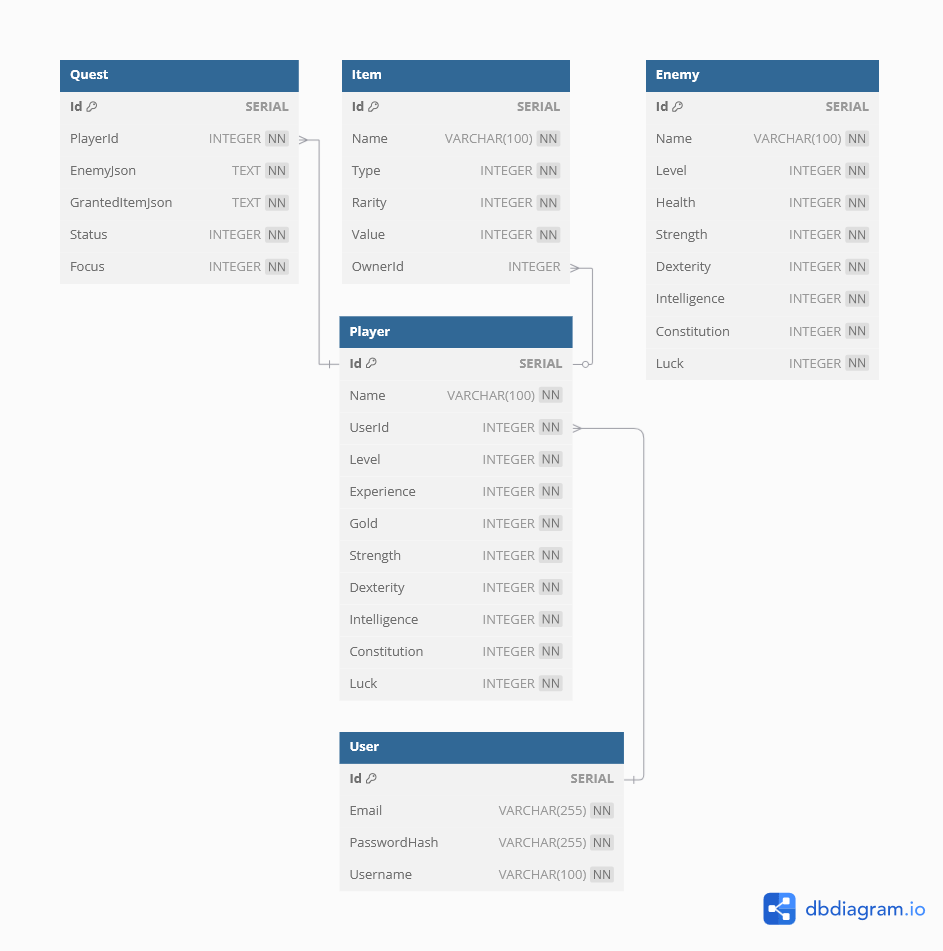
\includegraphics[width=0.8\textwidth]{figures/dbdiagram.png}
   \caption{Diagram bazy danych}
\end{figure}


% ********** Koniec rozdziału **********

% ********** Rozdział 4 **********
\chapter{Diagram przypadków użycia UML}

Na rysunku 3.2 przedstawiono diagram przypadków użycia systemu, ilustrujący główne interakcje użytkownika (gracza) z aplikacją.

\begin{figure}[h]
   \centering
   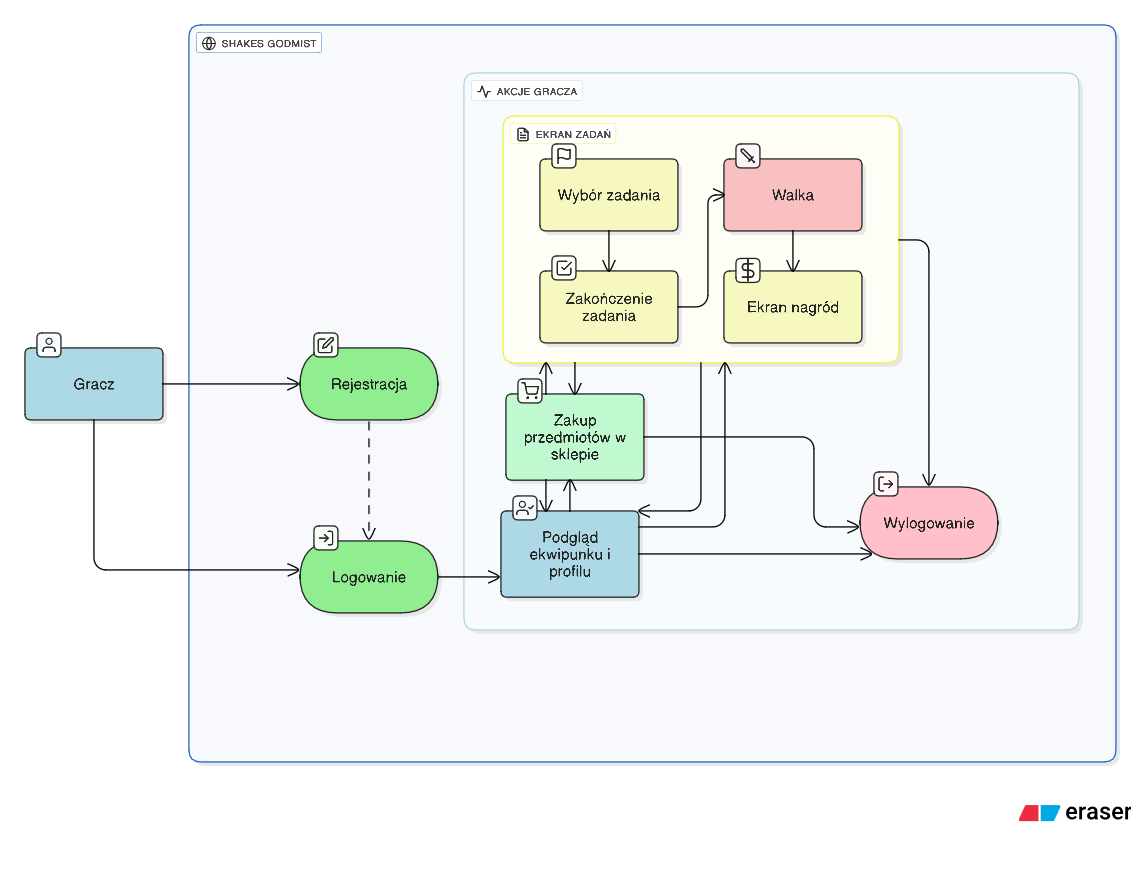
\includegraphics[width=0.8\textwidth]{figures/umldiagram.png}
   \caption{Diagram przypadków użycia UML}
\end{figure}

% ********** Koniec rozdziału **********

% ********** Rozdział 5 **********

\chapter{Opis kluczowych elementów back-endu}

W tej sekcji opisano najważniejsze elementy warstwy back-endowej projektu, ich odpowiedzialności oraz sposób działania.

\begin{itemize}
    \item \textbf{GameDbContext} -- Główny kontekst bazy danych, odpowiada za połączenie z bazą PostgreSQL oraz mapowanie encji (Player, Item, Quest, User, Enemy) na tabele w bazie. Umożliwia wykonywanie operacji CRUD na wszystkich obiektach domenowych. Konfiguracja relacji i kluczy obcych odbywa się w metodzie \texttt{OnModelCreating}. DbContext jest wykorzystywany przez wszystkie kontrolery do komunikacji z bazą danych.

    \item \textbf{AuthController} -- Odpowiada za obsługę rejestracji, logowania i uwierzytelniania użytkowników. Główne metody:
    \begin{itemize}
        \item \texttt{Register} -- rejestracja nowego użytkownika, walidacja danych, wywołanie serwisu AuthService.
        \item \texttt{Login} -- logowanie użytkownika, sprawdzenie poprawności hasła, generowanie tokenu JWT.
        \item \texttt{GetCurrentUser} -- pobranie danych aktualnie zalogowanego użytkownika na podstawie tokenu.
    \end{itemize}
    Kontroler komunikuje się z serwisem AuthService i zwraca odpowiedzi HTTP.

    \item \textbf{ItemsController} -- Zarządza operacjami na przedmiotach gracza. Główne metody:
    \begin{itemize}
        \item \texttt{GetItems} -- pobiera listę przedmiotów gracza.
        \item \texttt{BuyItem} -- umożliwia zakup nowego przedmiotu przez gracza, sprawdza saldo i dostępność.
        \item \texttt{SellItem} -- pozwala sprzedać przedmiot z ekwipunku gracza.
        \item \texttt{EquipItem} -- przypisuje przedmiot do slotu ekwipunku gracza.
    \end{itemize}
    Każda metoda waliduje uprawnienia użytkownika i wykonuje operacje na bazie przez GameDbContext.

    \item \textbf{PlayersController} -- Obsługuje operacje związane z graczem. Główne metody:
    \begin{itemize}
        \item \texttt{GetPlayer} -- pobiera profil i statystyki gracza.
        \item \texttt{UpgradeStats} -- umożliwia ulepszanie statystyk gracza, sprawdza koszty i limity.
        \item \texttt{GetInventory} -- pobiera ekwipunek gracza.
        \item \texttt{UpdatePlayer} -- aktualizuje dane gracza (np. po walce lub misji).
    \end{itemize}
    Kontroler sprawdza uprawnienia, pobiera i aktualizuje dane gracza w bazie, wywołuje logikę biznesową.

    \item \textbf{QuestsController} -- Odpowiada za generowanie, akceptowanie i kończenie misji. Główne metody:
    \begin{itemize}
        \item \texttt{GenerateQuests} -- generuje nowe propozycje misji na podstawie poziomu gracza.
        \item \texttt{AcceptQuest} -- przypisuje wybraną misję do gracza, serializuje przeciwnika i nagrodę.
        \item \texttt{CompleteQuest} -- kończy misję, przyznaje nagrody, aktualizuje postęp gracza.
        \item \texttt{GetActiveQuests} -- pobiera aktualne misje gracza.
    \end{itemize}
    Kontroler waliduje dostępność misji, uprawnienia gracza i zapisuje postęp w bazie.

    \item \textbf{AuthService} -- Serwis odpowiedzialny za logikę uwierzytelniania. Główne metody:
    \begin{itemize}
        \item \texttt{RegisterUser} -- tworzy nowego użytkownika, hashuje hasło, zapisuje w bazie.
        \item \texttt{ValidateUser} -- sprawdza poprawność danych logowania.
        \item \texttt{GenerateJwtToken} -- generuje token JWT dla zalogowanego użytkownika.
    \end{itemize}
    Oddziela logikę biznesową od kontrolera, zapewnia bezpieczeństwo i enkapsulację operacji na użytkownikach.

    \item \textbf{Podział odpowiedzialności} -- Logika biznesowa (np. generowanie misji, walidacja, przetwarzanie nagród) znajduje się po stronie back-endu, natomiast kontrolery odpowiadają za obsługę żądań HTTP i komunikację z klientem. Dane są przechowywane w bazie PostgreSQL, a dostęp do nich realizowany jest przez Entity Framework Core. Każdy kontroler odpowiada za walidację uprawnień i poprawności danych wejściowych.
\end{itemize}

% ********** Koniec rozdziału **********


% ********** Rozdział 6 **********
\chapter{Przypadki testowe}

W tej sekcji opisano przykładowe przypadki testowe dla kluczowych funkcjonalności systemu, zarówno po stronie backendu (API), jak i frontendu (interfejs użytkownika).

\section{Testy backendu (API)}

\begin{itemize}
    \item \textbf{Rejestracja nowego użytkownika}
    \begin{itemize}
        \item \textbf{Cel:} Sprawdzenie poprawności rejestracji użytkownika przez API.
        \item \textbf{Warunki początkowe:} Brak użytkownika o podanym e-mailu w bazie.
        \item \textbf{Kroki testowe:}
        \begin{enumerate}
            \item Wysłanie żądania POST /api/auth/register z danymi użytkownika.
        \end{enumerate}
        \item \textbf{Dane wejściowe:} Przykładowy e-mail, hasło, nazwa użytkownika.
        \item \textbf{Oczekiwany rezultat:} Odpowiedź 200 OK, utworzenie nowego użytkownika w bazie.
        \item \textbf{Wynik testu:}
        \begin{figure}[H]
            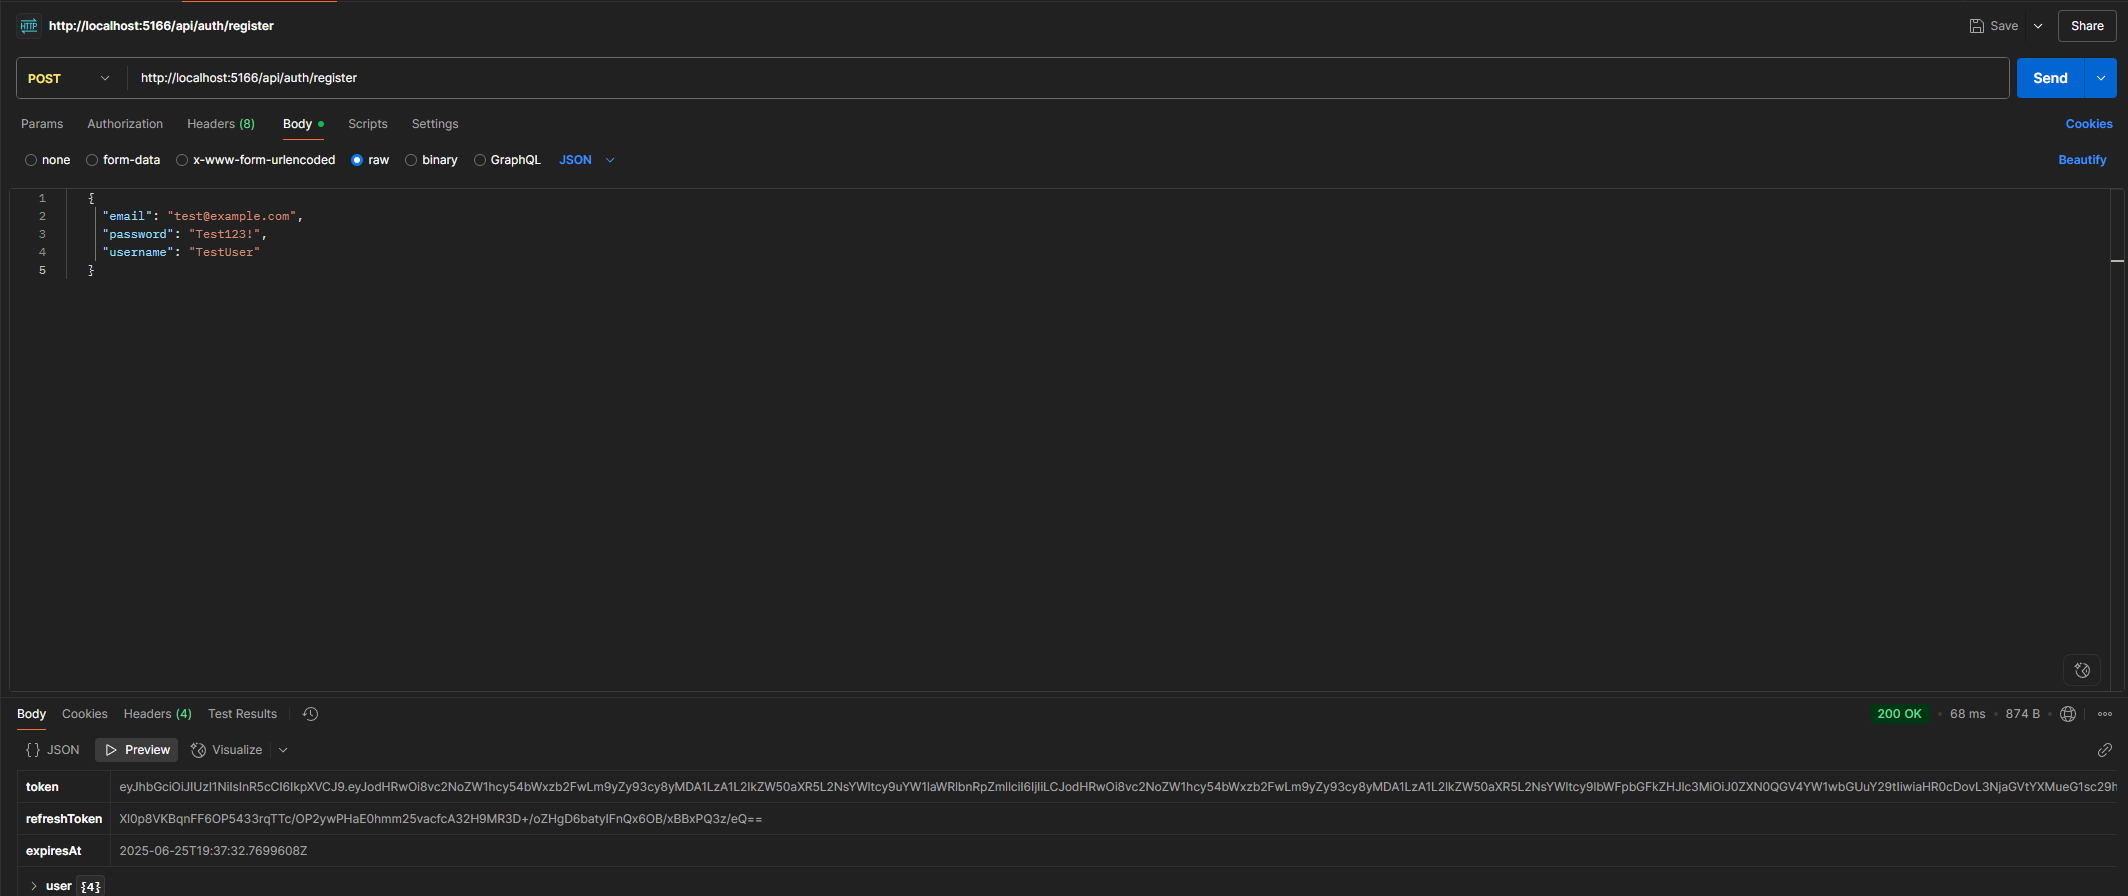
\includegraphics[width=480px]{figures/testy/test-registration.png}
            \caption{Test rejestracji użytkownika}
        \end{figure}
    \end{itemize}

    \item \textbf{Logowanie użytkownika}
    \begin{itemize}
        \item \textbf{Cel:} Sprawdzenie poprawności logowania i generowania tokenu JWT.
        \item \textbf{Warunki początkowe:} Istnieje użytkownik z podanym e-mailem i hasłem.
        \item \textbf{Kroki testowe:}
        \begin{enumerate}
            \item Wysłanie żądania POST /api/auth/login z poprawnymi danymi.
        \end{enumerate}
        \item \textbf{Dane wejściowe:} E-mail, hasło.
        \item \textbf{Oczekiwany rezultat:} Odpowiedź 200 OK, zwrócony token JWT.
        \item \textbf{Wynik testu:}
        \begin{figure}[H]
            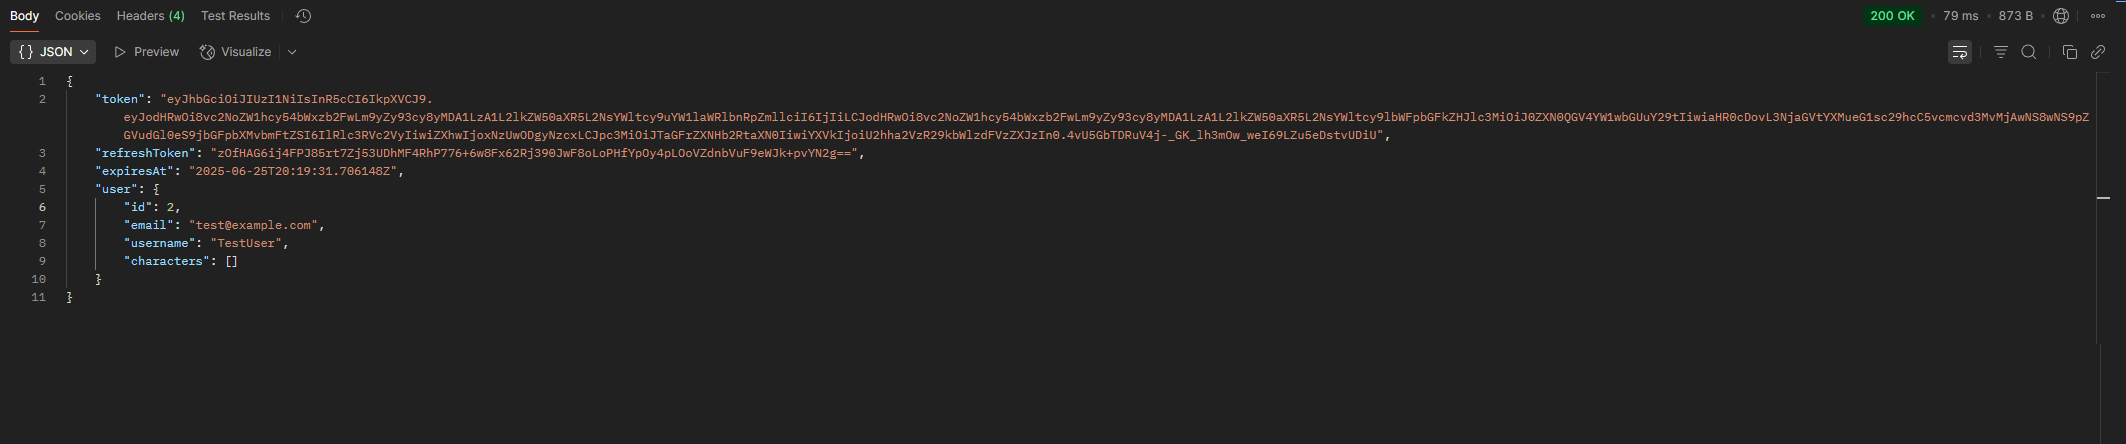
\includegraphics[width=480px]{figures/testy/test-login.png}
            \caption{Test logowania użytkownika}
        \end{figure}
    \end{itemize}

    \item \textbf{Pobranie profilu gracza}
    \begin{itemize}
        \item \textbf{Cel:} Sprawdzenie możliwości pobrania danych gracza.
        \item \textbf{Warunki początkowe:} Użytkownik jest zalogowany (ma token JWT).
        \item \textbf{Kroki testowe:}
        \begin{enumerate}
            \item Wysłanie żądania GET /api/players z nagłówkiem Authorization: Bearer <token>.
        \end{enumerate}
        \item \textbf{Dane wejściowe:} Token JWT.
        \item \textbf{Oczekiwany rezultat:} Odpowiedź 200 OK, zwrócone dane gracza.
        \item \textbf{Wynik testu:}
        \begin{figure}[H]
            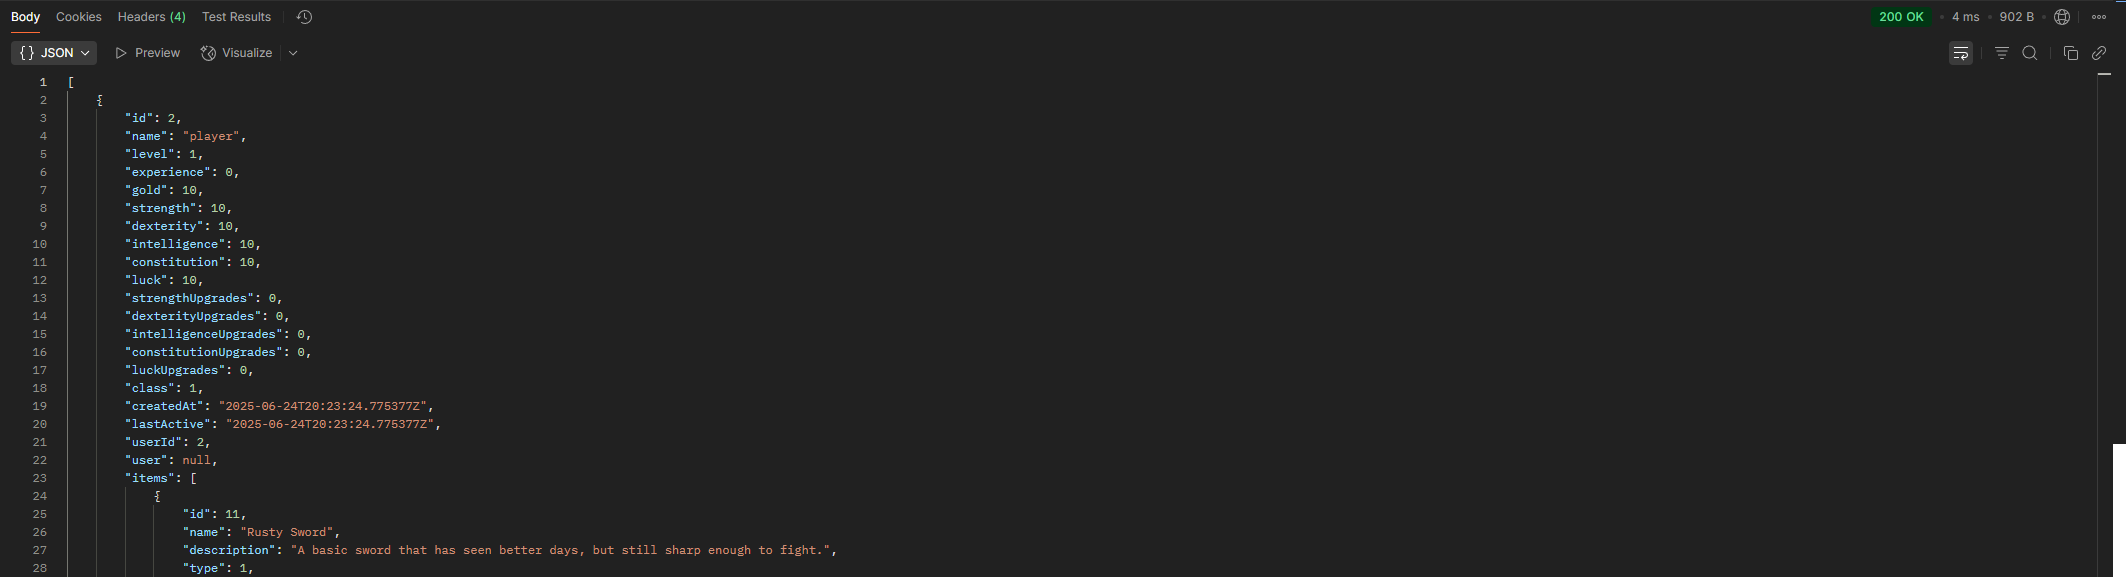
\includegraphics[width=480px]{figures/testy/test-playerdata.png}
            \caption{Test danych gracza}
        \end{figure}
    \end{itemize}

    \item \textbf{Zakup przedmiotu}
    \begin{itemize}
        \item \textbf{Cel:} Sprawdzenie możliwości zakupu przedmiotu przez API.
        \item \textbf{Warunki początkowe:} Gracz jest zalogowany, ma wystarczającą ilość złota.
        \item \textbf{Kroki testowe:}
        \begin{enumerate}
            \item Wysłanie żądania POST /api/items/buy z danymi przedmiotu.
        \end{enumerate}
        \item \textbf{Dane wejściowe:} Identyfikator przedmiotu, token JWT.
        \item \textbf{Oczekiwany rezultat:} Odpowiedź 400 Bad Request, gracz nie ma wystarczającej ilości złota.
        \item \textbf{Wynik testu:}
        \begin{figure}[H]
            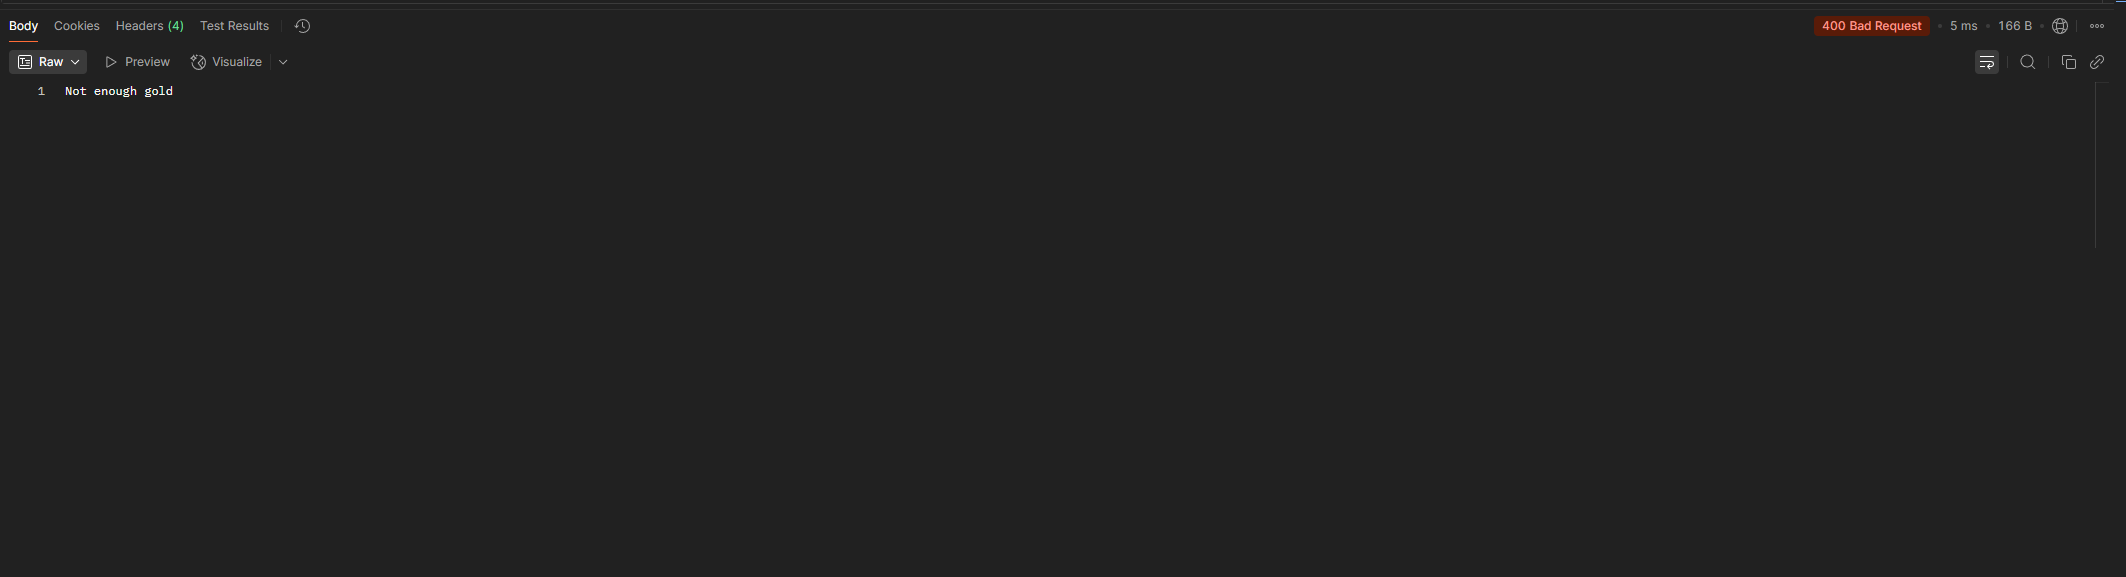
\includegraphics[width=480px]{figures/testy/test-buyitem-fail.png}
            \caption{Test zakupu przedmiotu - brak złota}
        \end{figure}
    \end{itemize}

    \item \textbf{Rozpoczęcie nowej misji}
    \begin{itemize}
        \item \textbf{Cel:} Sprawdzenie możliwości rozpoczęcia misji przez API.
        \item \textbf{Warunki początkowe:} Gracz jest zalogowany, ma dostępne misje.
        \item \textbf{Kroki testowe:}
        \begin{enumerate}
            \item Wysłanie żądania POST /api/quests/start z danymi misji.
        \end{enumerate}
        \item \textbf{Dane wejściowe:} Identyfikator misji, token JWT.
        \item \textbf{Oczekiwany rezultat:} Odpowiedź 200 OK, misja przypisana do gracza.
        \item \textbf{Wynik testu:}
        \begin{figure}[H]
            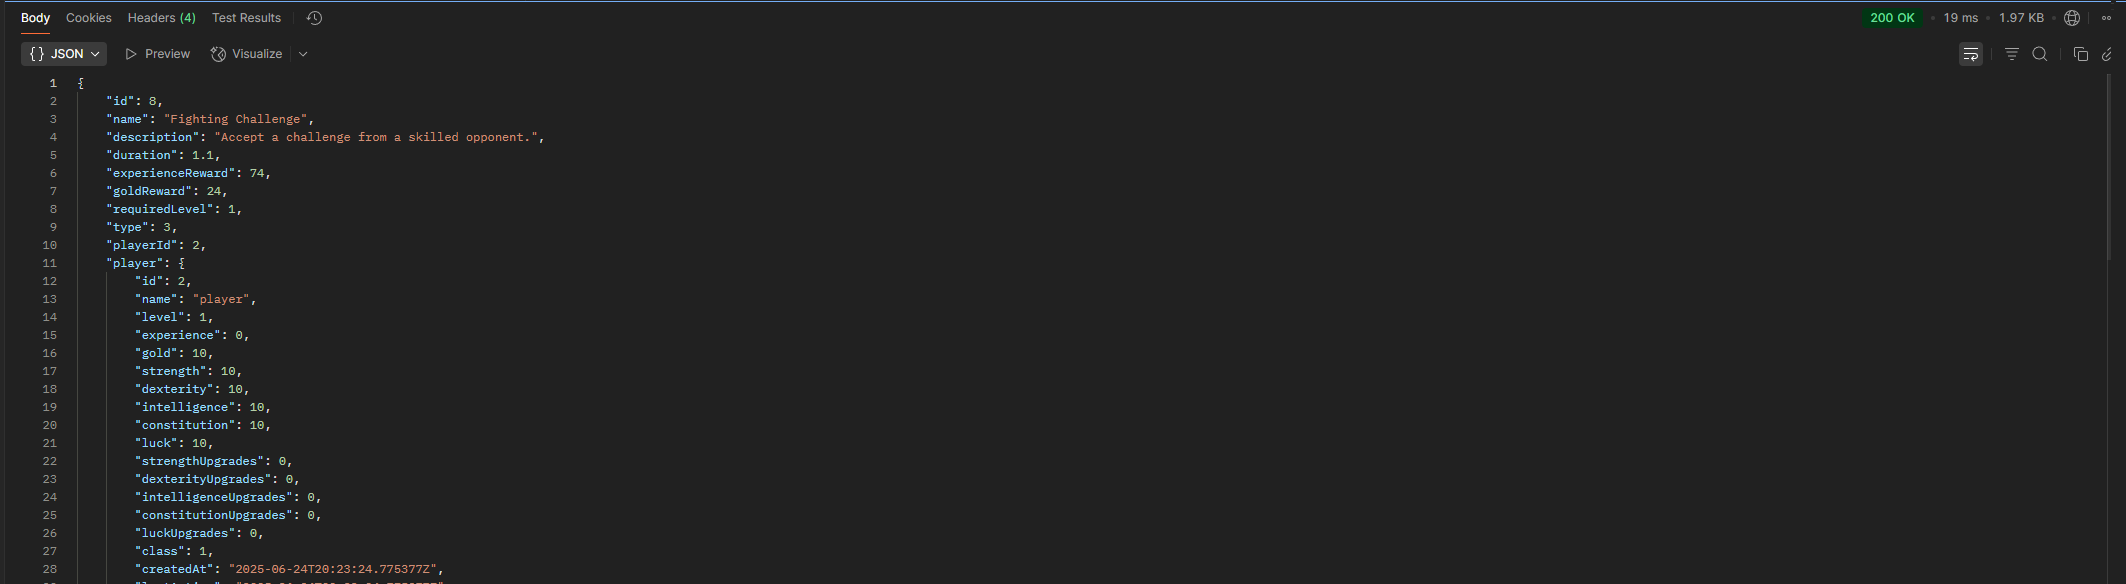
\includegraphics[width=480px]{figures/testy/test-startquest.png}
            \caption{Test rozpoczęcia misji}
        \end{figure}
    \end{itemize}

    \item \textbf{Zakończenie misji}
    \begin{itemize}
        \item \textbf{Cel:} Sprawdzenie poprawności zakończenia misji i przyznania nagrody.
        \item \textbf{Warunki początkowe:} Gracz ma aktywną misję.
        \item \textbf{Kroki testowe:}
        \begin{enumerate}
            \item Wysłanie żądania POST /api/quests/complete z danymi misji.
        \end{enumerate}
        \item \textbf{Dane wejściowe:} Identyfikator misji, token JWT.
        \item \textbf{Oczekiwany rezultat:} Odpowiedź 200 OK, nagroda dodana do ekwipunku, XP i złoto zaktualizowane.
        \item \textbf{Wynik testu:}
        \begin{figure}[H]
            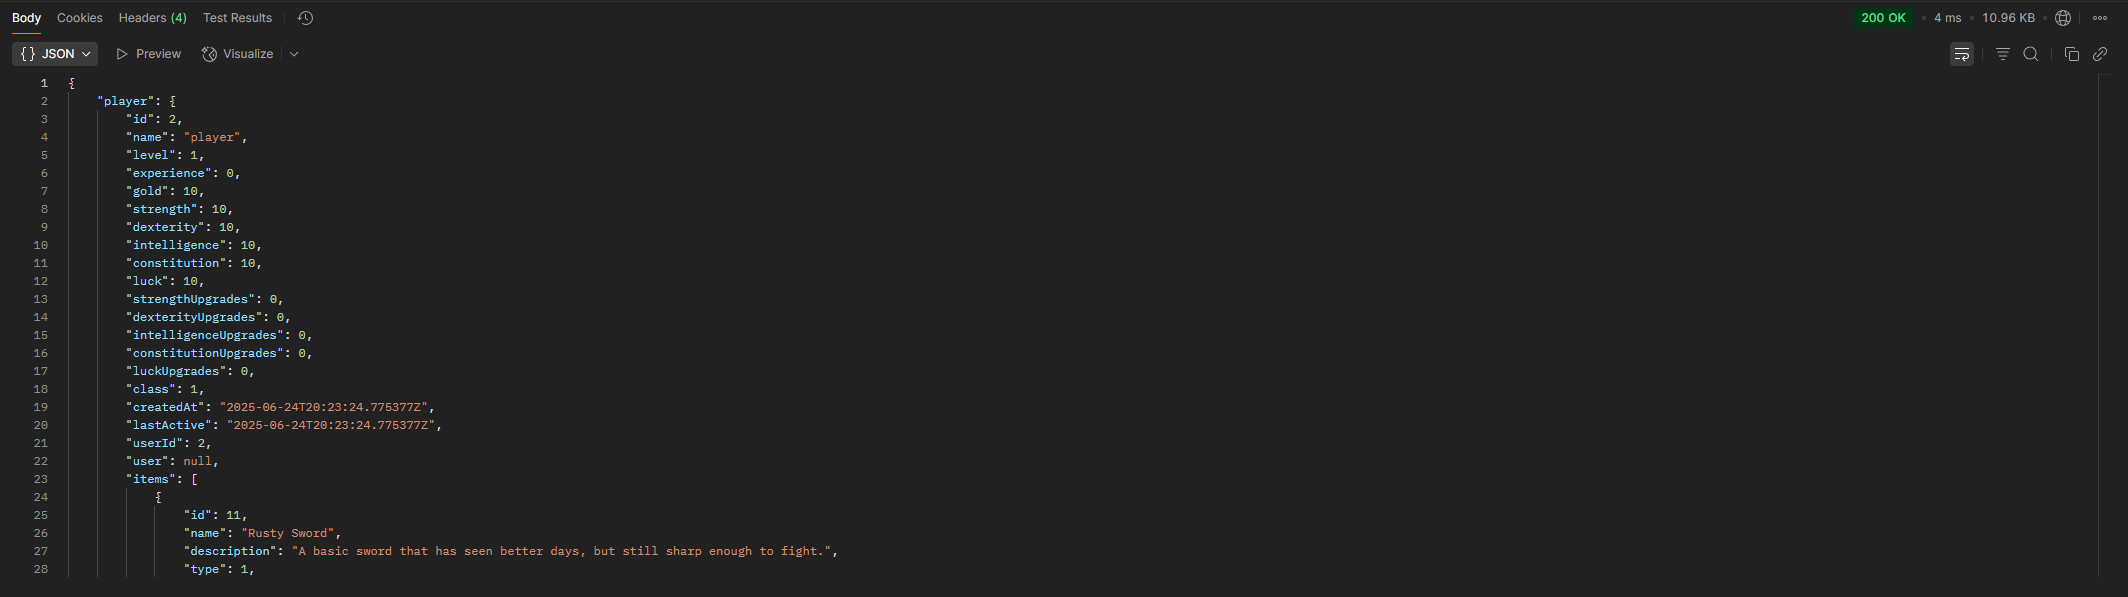
\includegraphics[width=480px]{figures/testy/test-completequest.png}
            \caption{Test zakończenia misji}
        \end{figure}
    \end{itemize}

    \item \textbf{Obsługa nieautoryzowanego dostępu}
    \begin{itemize}
        \item \textbf{Cel:} Sprawdzenie, czy API odrzuca żądania bez ważnego tokenu.
        \item \textbf{Warunki początkowe:} Brak tokenu lub token nieprawidłowy.
        \item \textbf{Kroki testowe:}
        \begin{enumerate}
            \item Wysłanie żądania GET /api/players/me bez nagłówka Authorization.
        \end{enumerate}
        \item \textbf{Dane wejściowe:} Brak lub nieprawidłowy token.
        \item \textbf{Oczekiwany rezultat:} Odpowiedź 401 Unauthorized.
        \item \textbf{Wynik testu:}
        \begin{figure}[H]
            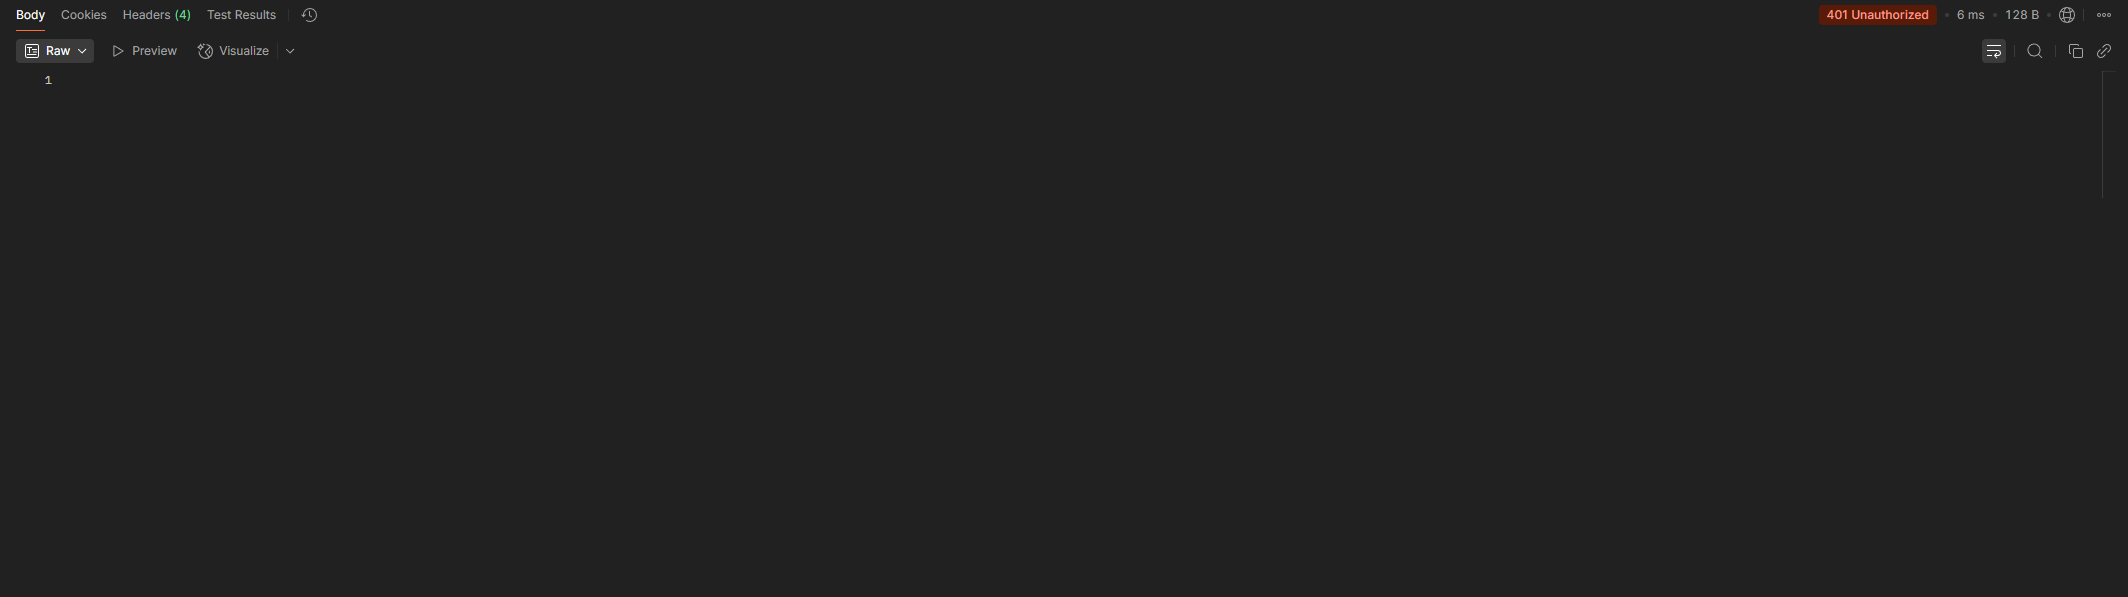
\includegraphics[width=480px]{figures/testy/test-unauthorized.png}
            \caption{Test nieautoryzowanego dostępu}
        \end{figure}
    \end{itemize}
\end{itemize}

\section{Testy frontendu (UI)}

\begin{itemize}
    \item \textbf{Rejestracja użytkownika przez interfejs}
    \begin{itemize}
        \item \textbf{Cel:} Sprawdzenie poprawności działania formularza rejestracji.
        \item \textbf{Warunki początkowe:} Brak zalogowanego użytkownika.
        \item \textbf{Kroki testowe:}
        \begin{enumerate}
            \item Otwórz stronę rejestracji.
            \item Wprowadź dane użytkownika i zatwierdź formularz.
        \end{enumerate}
        \item \textbf{Dane wejściowe:} E-mail, hasło, nazwa użytkownika.
        \item \textbf{Oczekiwany rezultat:} Komunikat o sukcesie, przekierowanie do ekranu logowania lub gry.
        \item \textbf{Wynik testu:}
        \begin{figure}[H]
            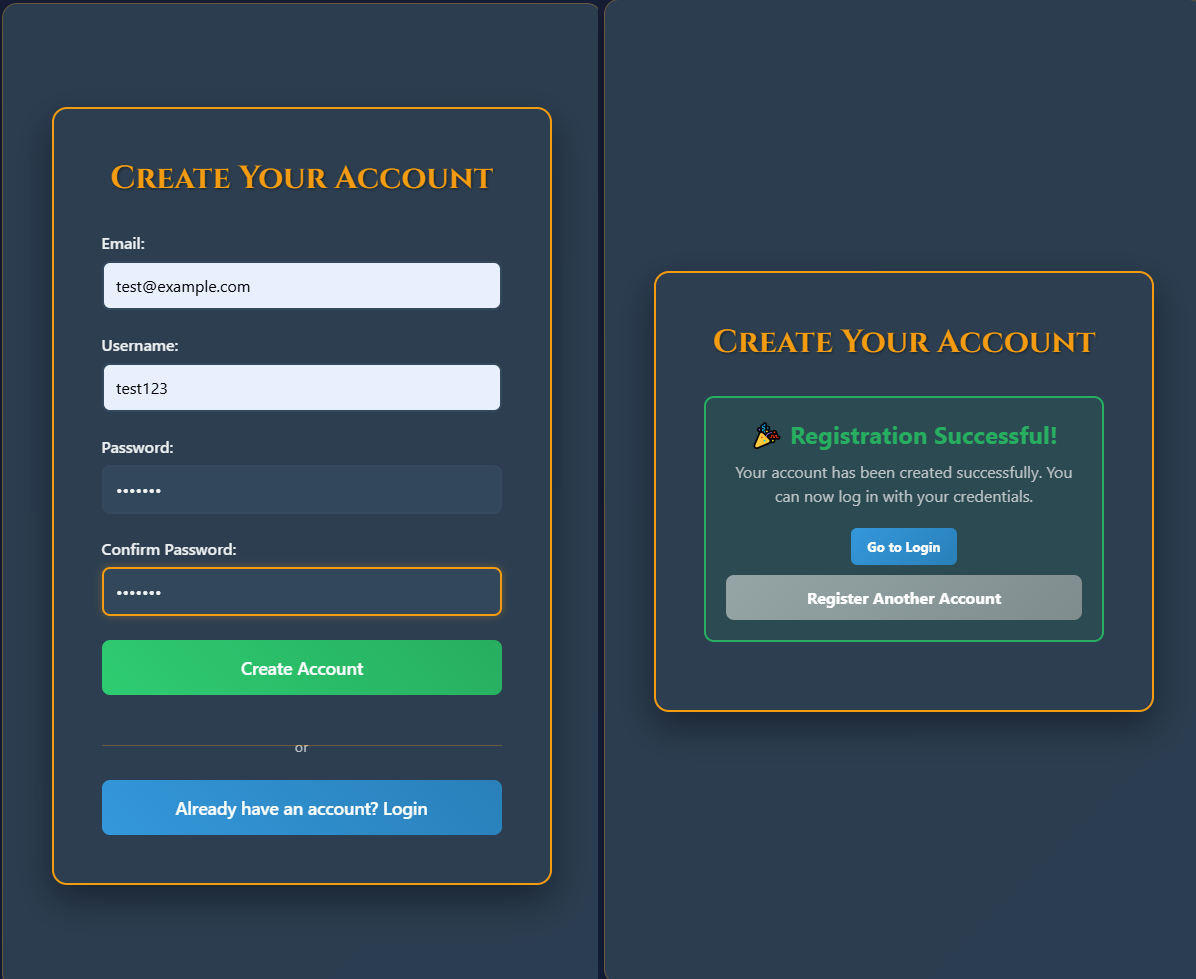
\includegraphics[width=480px]{figures/testy/test-registration-front.png}
            \caption{Test rejestracji użytkownika - frontend}
        \end{figure}
    \end{itemize}


    \item \textbf{Logowanie użytkownika przez interfejs}
    \begin{itemize}
        \item \textbf{Cel:} Sprawdzenie poprawności działania formularza logowania.
        \item \textbf{Warunki początkowe:} Istnieje zarejestrowany użytkownik.
        \item \textbf{Kroki testowe:}
        \begin{enumerate}
            \item Otwórz stronę logowania.
            \item Wprowadź poprawne dane i zatwierdź formularz.
        \end{enumerate}
        \item \textbf{Dane wejściowe:} E-mail, hasło.
        \item \textbf{Oczekiwany rezultat:} Przekierowanie do ekranu gry, widoczne dane gracza.
        \item \textbf{Wynik testu:}
        \begin{figure}[H]
            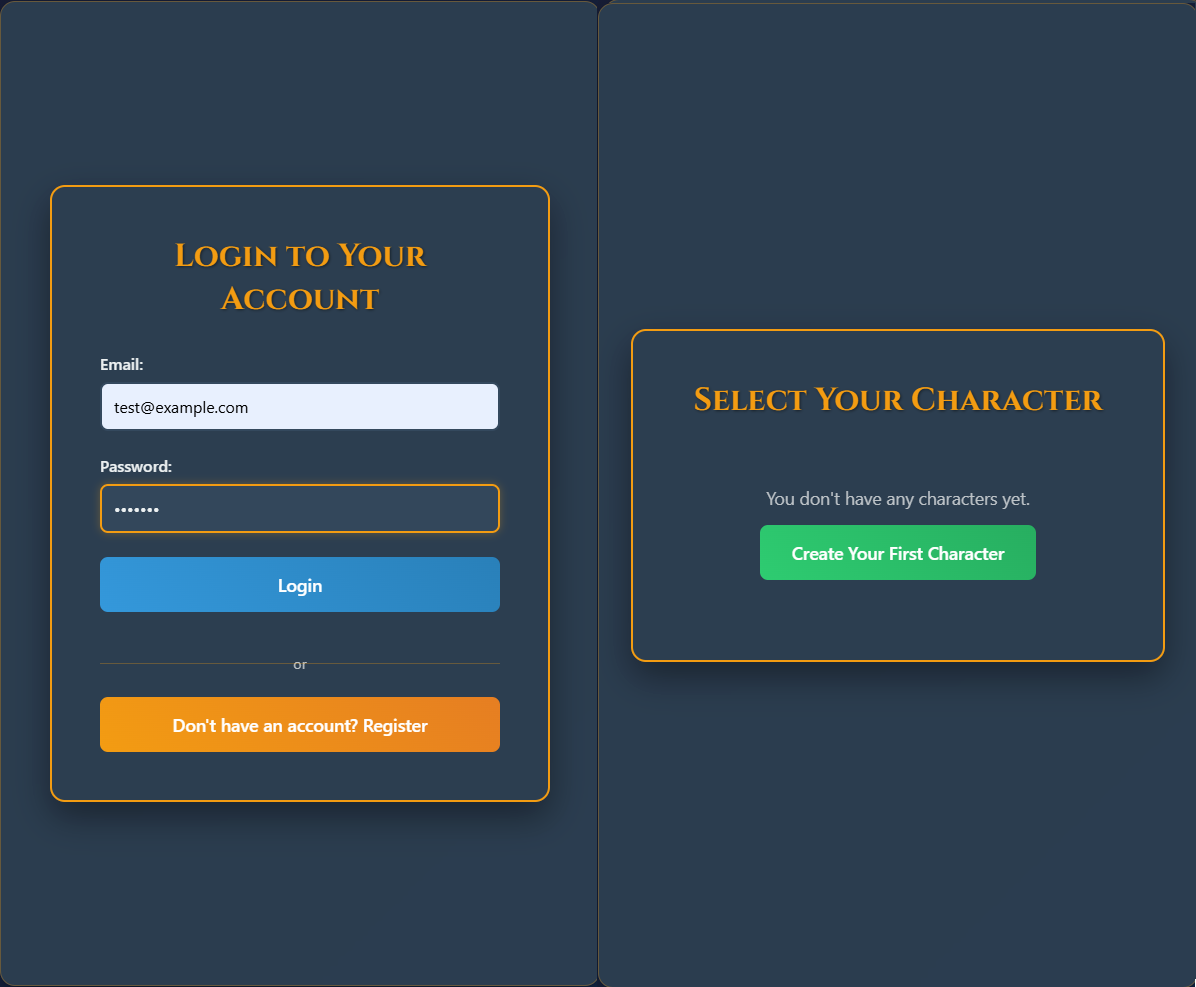
\includegraphics[width=480px]{figures/testy/test-login-front.png}
            \caption{Test logowania użytkownika - frontend}
        \end{figure}
    \end{itemize}

    \item \textbf{Wyświetlanie ekwipunku gracza}
    \begin{itemize}
        \item \textbf{Cel:} Sprawdzenie poprawności wyświetlania ekwipunku po zalogowaniu.
        \item \textbf{Warunki początkowe:} Gracz jest zalogowany, posiada przedmioty.
        \item \textbf{Kroki testowe:}
        \begin{enumerate}
            \item Przejdź do ekranu ekwipunku.
        \end{enumerate}
        \item \textbf{Dane wejściowe:} Token JWT (w tle).
        \item \textbf{Oczekiwany rezultat:} Lista przedmiotów widoczna na ekranie.
        \item \textbf{Wynik testu:}
        \begin{figure}[H]
            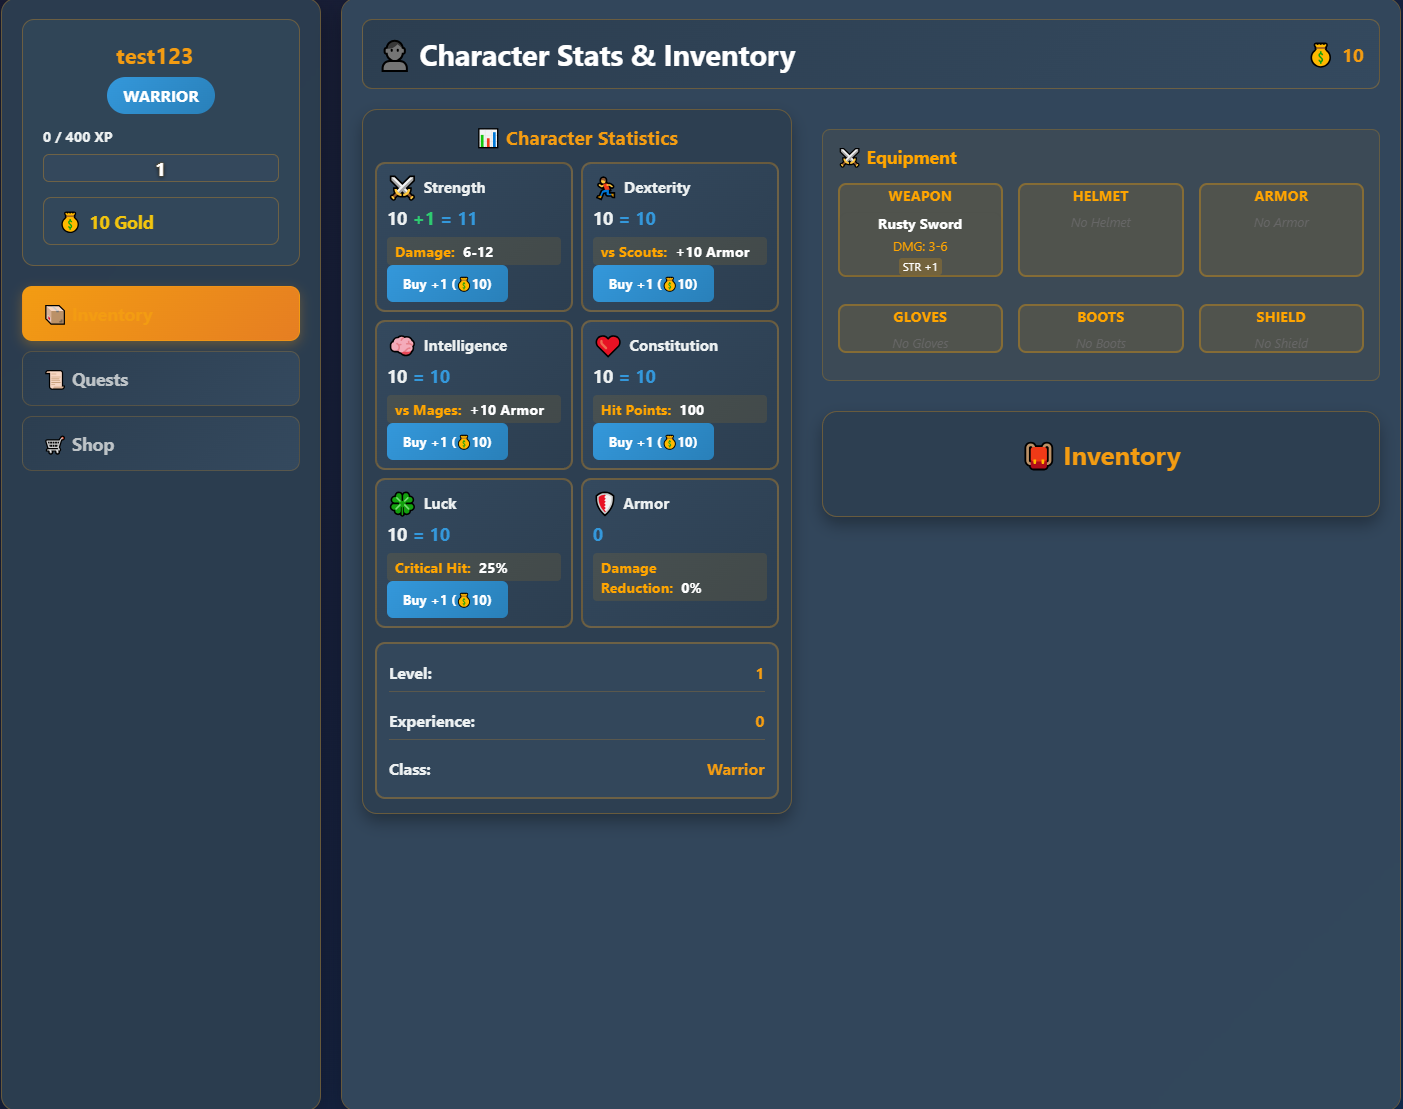
\includegraphics[width=480px]{figures/testy/test-inventory-front.png}
            \caption{Test ekwipunku gracza}
        \end{figure}
    \end{itemize}

    \item \textbf{Zakup przedmiotu przez interfejs}
    \begin{itemize}
        \item \textbf{Cel:} Sprawdzenie możliwości zakupu przedmiotu przez UI.
        \item \textbf{Warunki początkowe:} Gracz jest zalogowany, ma wystarczającą ilość złota.
        \item \textbf{Kroki testowe:}
        \begin{enumerate}
            \item Przejdź do sklepu.
            \item Wybierz przedmiot i kliknij "Kup".
        \end{enumerate}
        \item \textbf{Dane wejściowe:} Identyfikator przedmiotu (wybór w UI).
        \item \textbf{Oczekiwany rezultat:} Przedmiot pojawia się w ekwipunku, złoto zmniejszone.
        \item \textbf{Wynik testu:}
        \begin{figure}[H]
            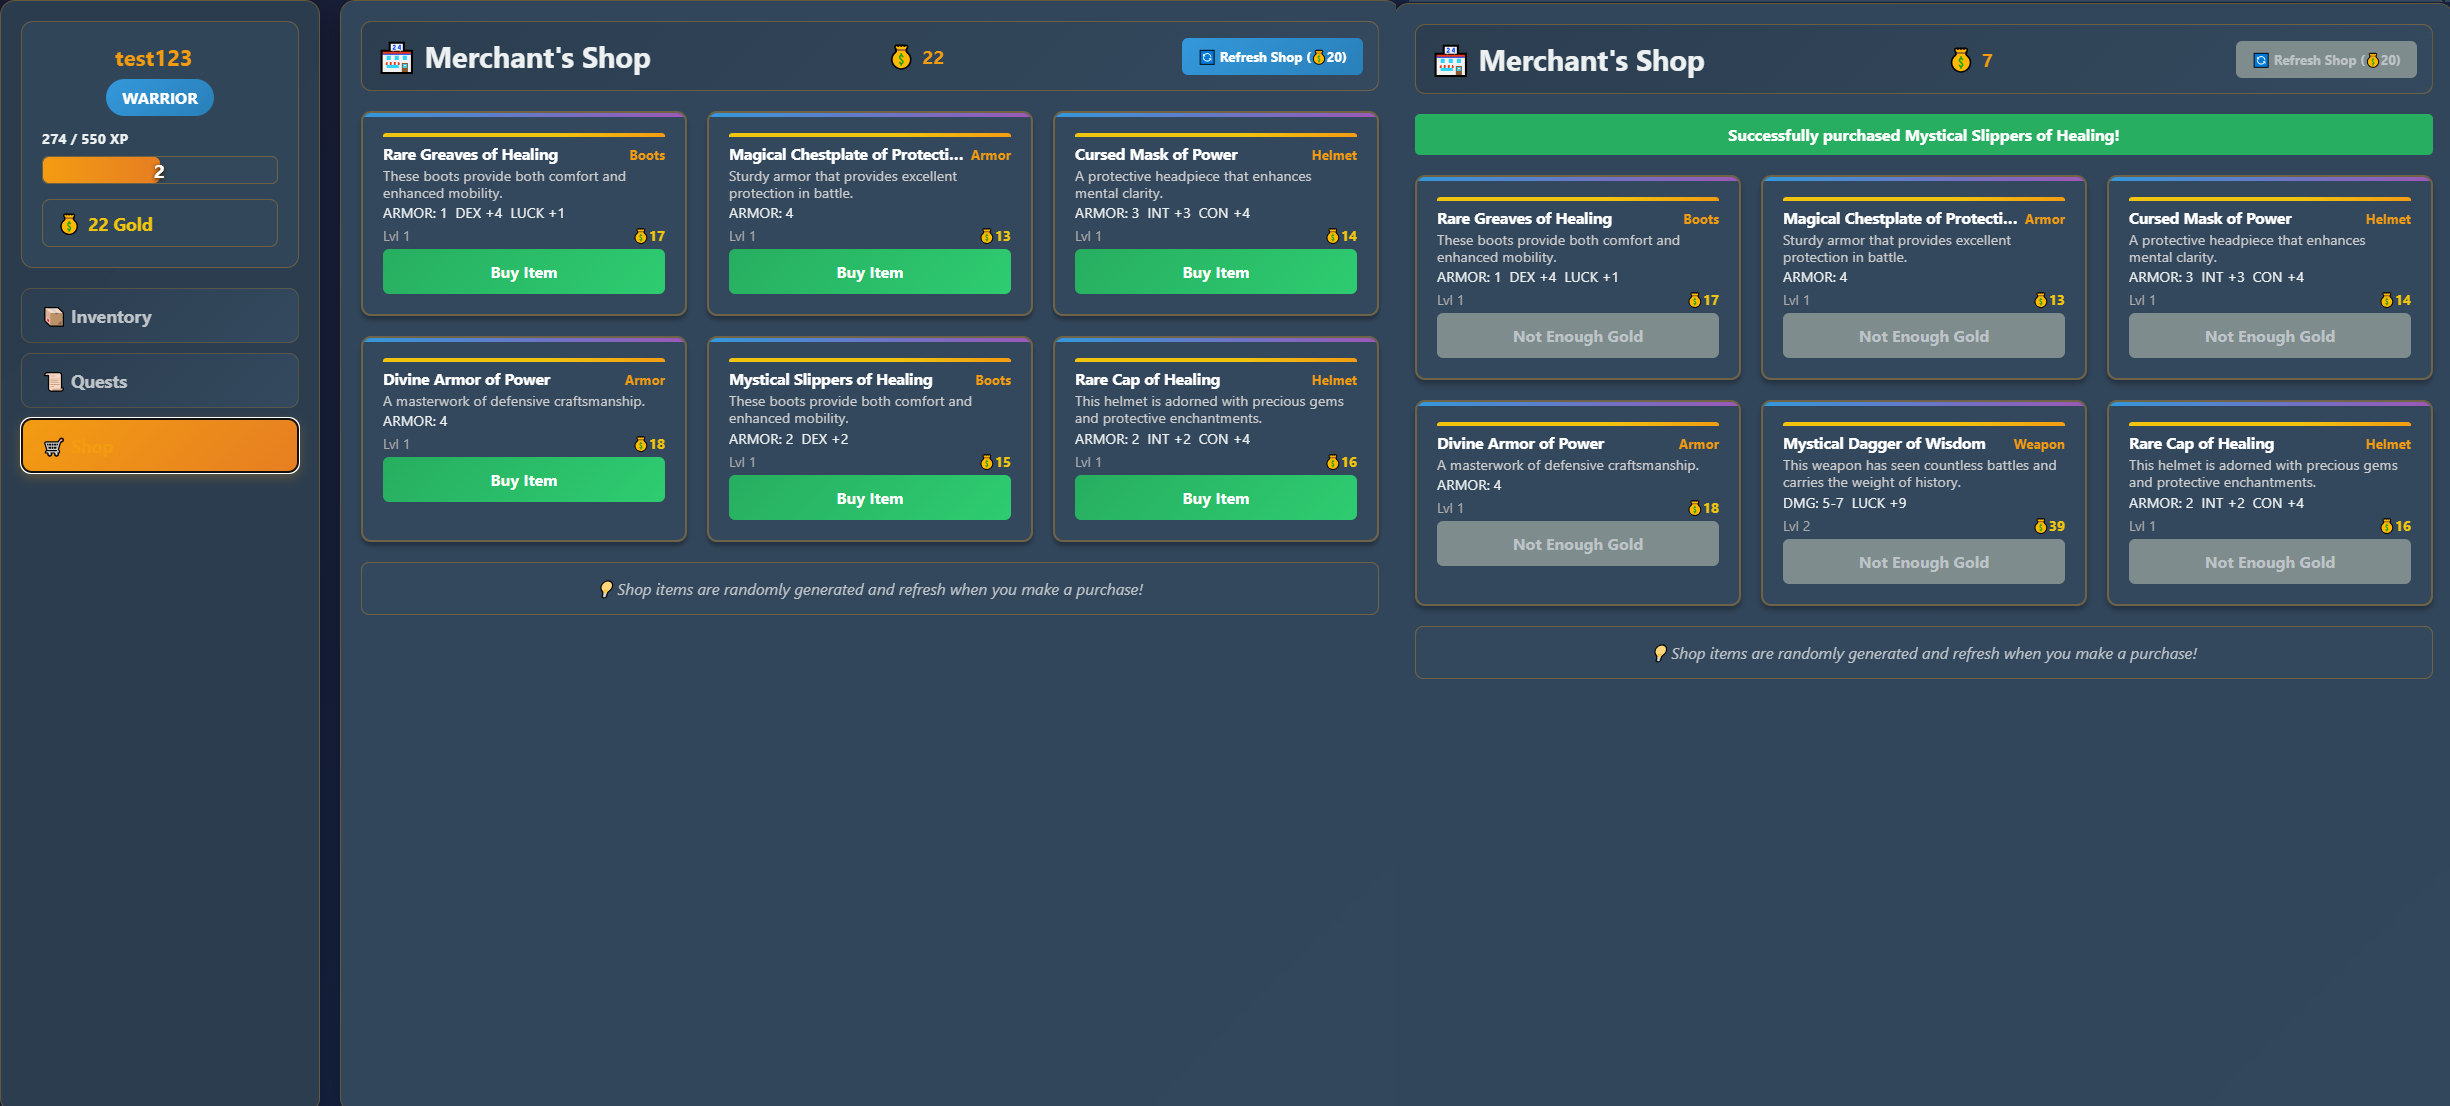
\includegraphics[width=480px]{figures/testy/test-buyitem-front.png}
            \caption{Test zakupu przedmiotu - frontend}
        \end{figure}
    \end{itemize}

    \item \textbf{Rozpoczęcie i zakończenie misji przez interfejs}
    \begin{itemize}
        \item \textbf{Cel:} Sprawdzenie poprawności obsługi misji przez UI.
        \item \textbf{Warunki początkowe:} Gracz jest zalogowany, ma dostępne misje.
        \item \textbf{Kroki testowe:}
        \begin{enumerate}
            \item Przejdź do tablicy misji.
            \item Wybierz misję i kliknij "Rozpocznij".
            \item Po zakończeniu kliknij "Odbierz nagrodę".
        \end{enumerate}
        \item \textbf{Dane wejściowe:} Identyfikator misji (wybór w UI).
        \item \textbf{Oczekiwany rezultat:} Misja znika z listy aktywnych, nagroda pojawia się w ekwipunku.
        \item \textbf{Wynik testu:}
        \begin{figure}[H]
            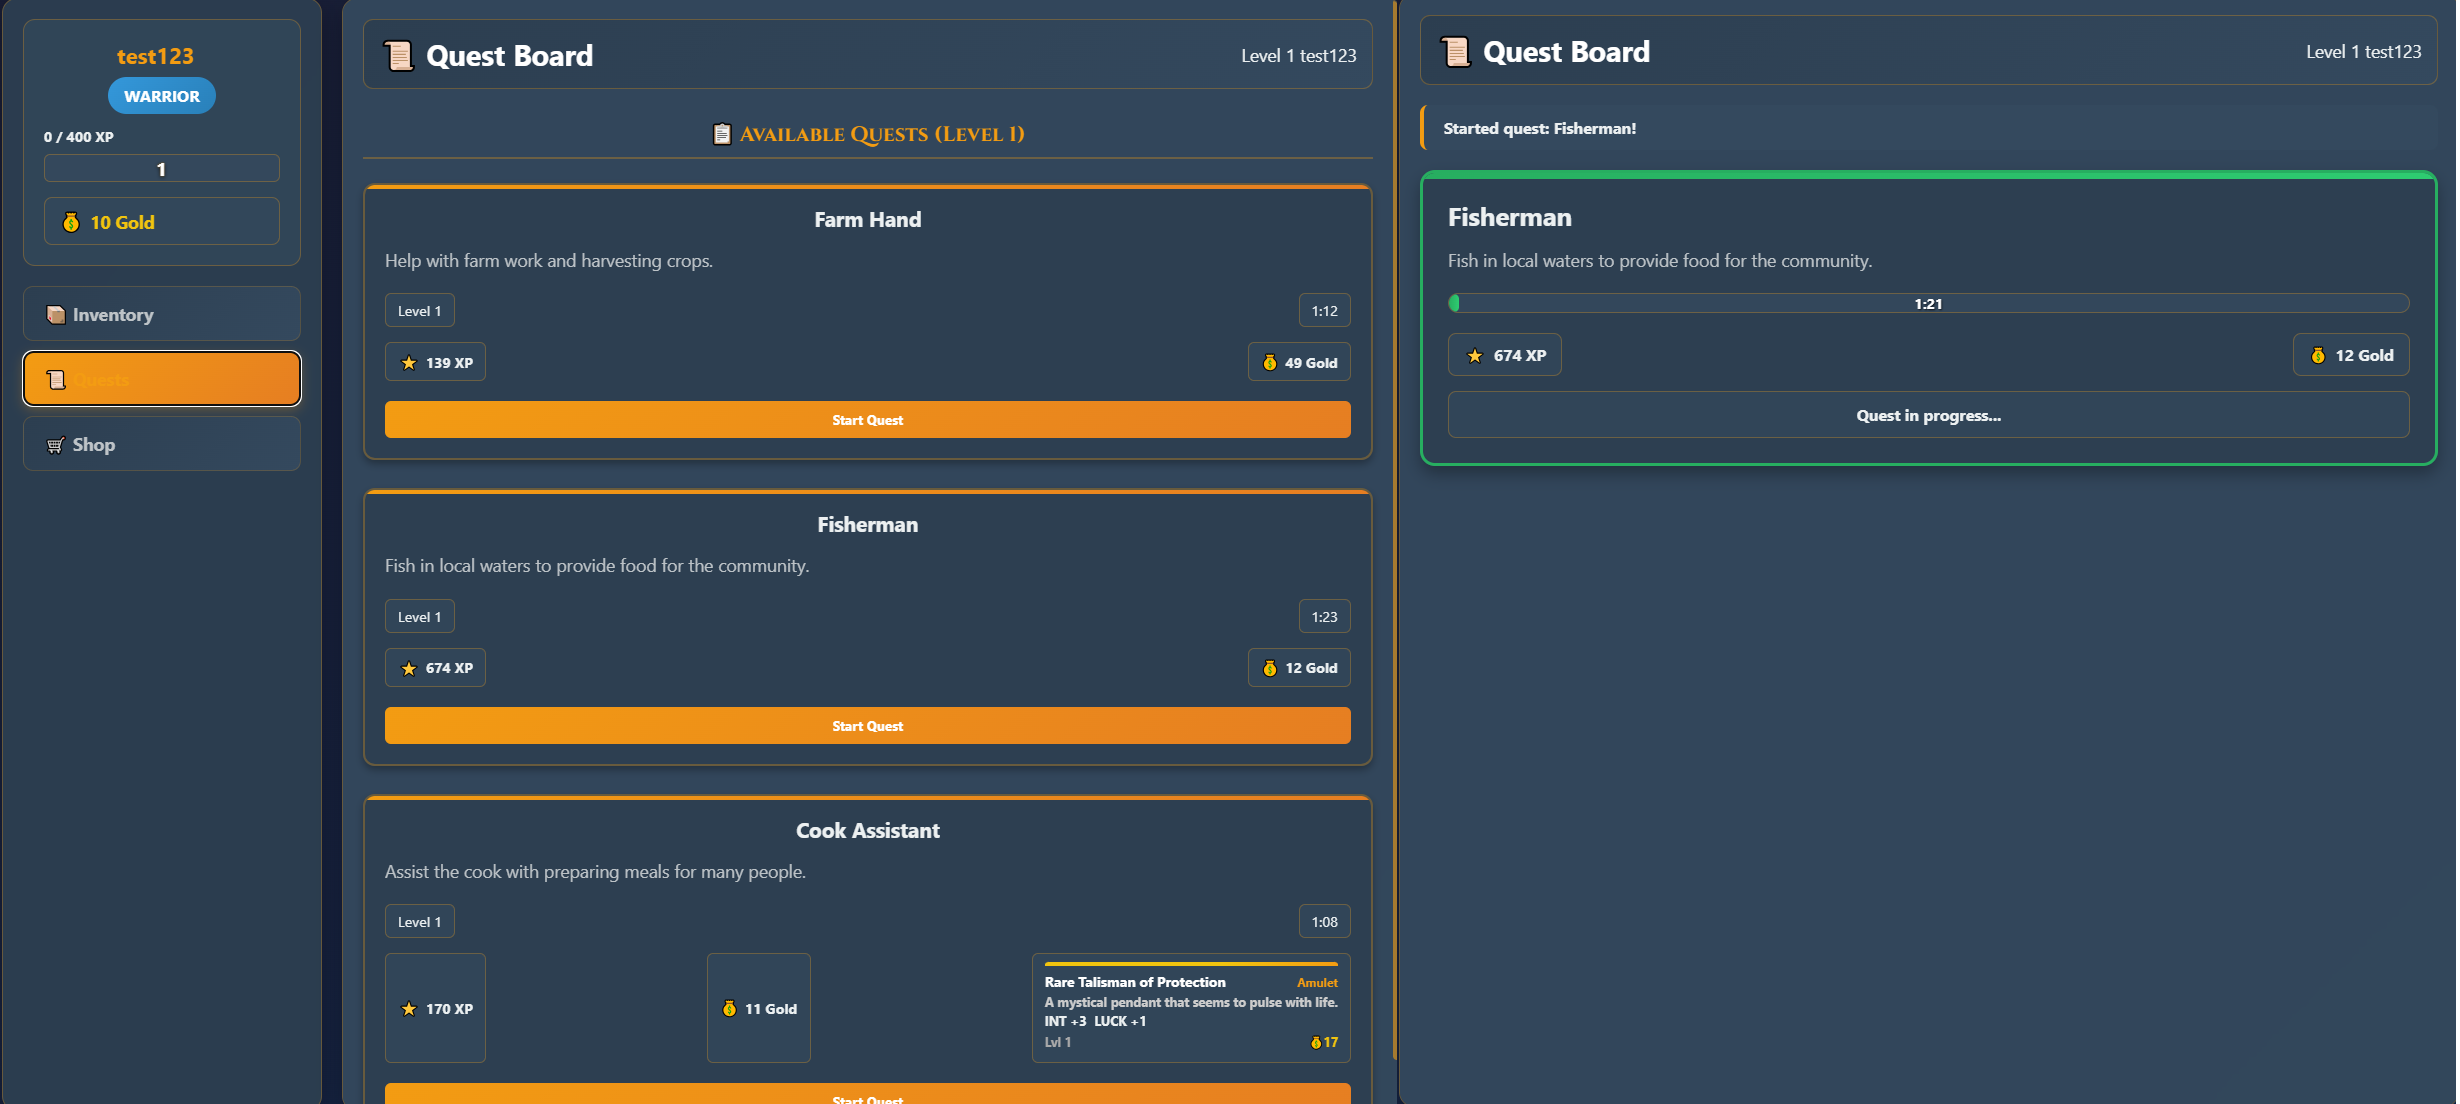
\includegraphics[width=480px]{figures/testy/test-startquest-front.png}
            \caption{Test rozpoczęcia misji}
        \end{figure}
        \begin{figure}[H]
            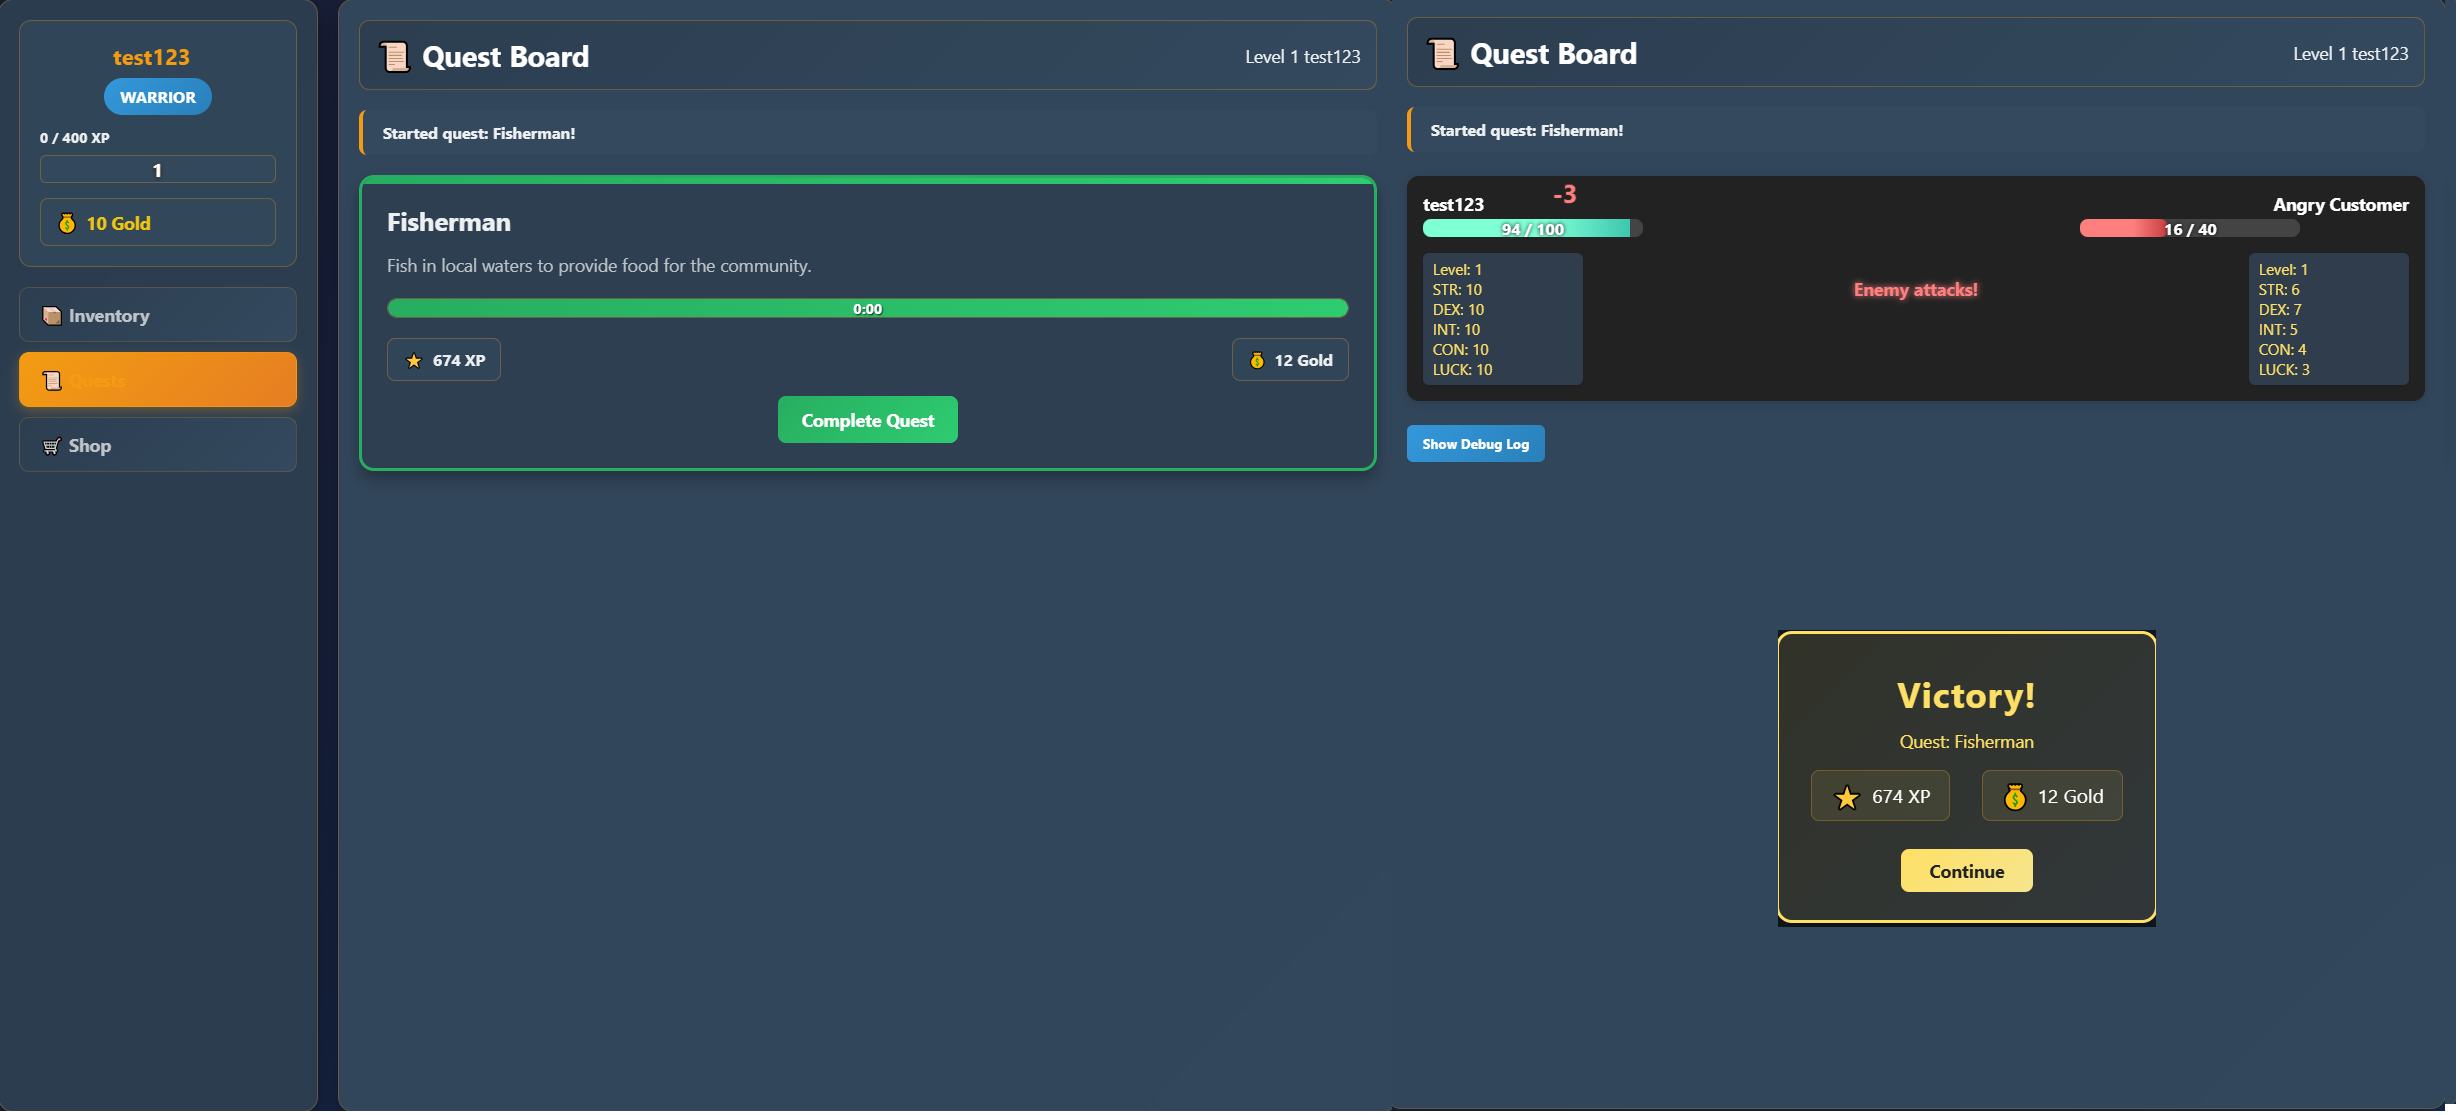
\includegraphics[width=480px]{figures/testy/test-completequest-front.png}
            \caption{Test zakończenia misji}
        \end{figure}
    \end{itemize}

    \item \textbf{Ulepszenie statystyk przez interfejs}
    \begin{itemize}
        \item \textbf{Cel:} Sprawdzenie możliwości ulepszania statystyk przez UI.
        \item \textbf{Warunki początkowe:} Gracz jest zalogowany, ma wystarczającą ilość złota.
        \item \textbf{Kroki testowe:}
        \begin{enumerate}
            \item Przejdź do ekranu statystyk.
            \item Kliknij przycisk ulepszenia wybranej statystyki.
        \end{enumerate}
        \item \textbf{Dane wejściowe:} Nazwa statystyki (wybór w UI).
        \item \textbf{Oczekiwany rezultat:} Statystyka zwiększona, złoto zmniejszone.
        \item \textbf{Wynik testu:}
        \begin{figure}[H]
            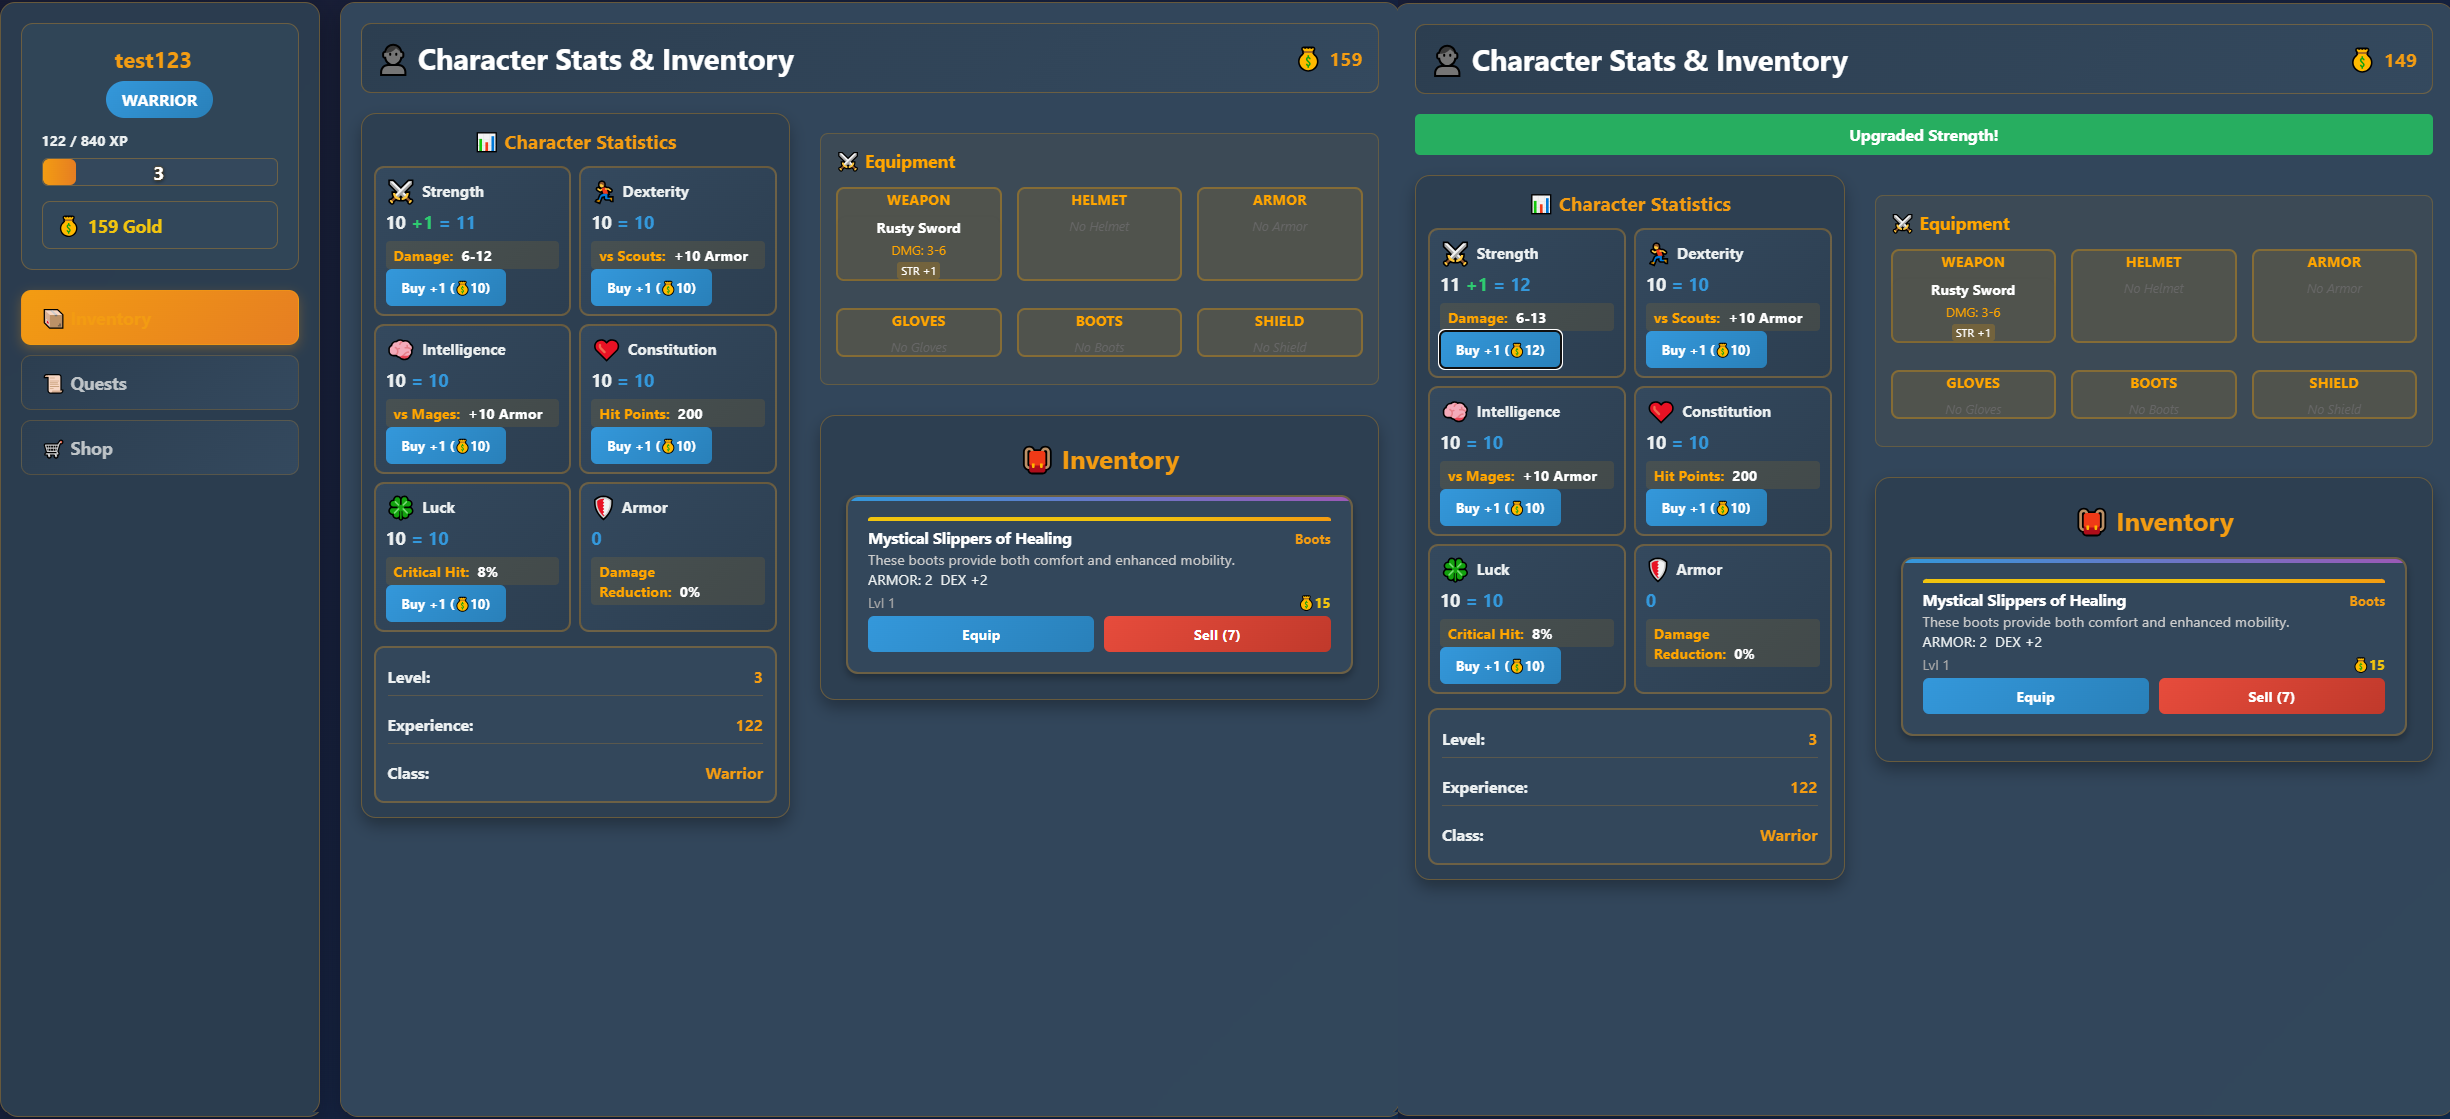
\includegraphics[width=480px]{figures/testy/test-upgradestat-front.png}
            \caption{Test ulepszenia statystyk}
        \end{figure}
    \end{itemize}
\end{itemize}



% ********** Koniec rozdziału **********
\chapter{Planowane place rozwojowe}

W tej sekcji opisano kierunki rozwoju systemu, które mogą być zaimplementowane w przyszłych wersjach aplikacji.

\section{Rozszerzenia funkcjonalności gry}

\begin{itemize}
    \item \textbf{System klanów i gildii}
    \begin{itemize}
        \item Tworzenie i zarządzanie klanami przez graczy
        \item Wspólne misje klanowe z większymi nagrodami
        \item System rankingowy klanów
        \item Czat wewnętrzny klanu
    \end{itemize}

    \item \textbf{System PvP (Player vs Player)}
    \begin{itemize}
        \item Areny PvP z rankingiem graczy
        \item Turnieje sezonowe z nagrodami
        \item System wyzwań między graczami
        \item Specjalne przedmioty dostępne tylko w PvP
    \end{itemize}

    \item \textbf{Rozszerzony system przedmiotów}
    \begin{itemize}
        \item System rzadkości przedmiotów (pospolite, rzadkie, epickie, legendarne)
        \item System enchantów i run
        \item Kolekcjonowanie zestawów przedmiotów z bonusami
        \item Skalowanie statystyk z poziomem
    \end{itemize}

    \item \textbf{System osiągnięć}
    \begin{itemize}
        \item Osiągnięcia za różne działania w grze
        \item System punktów prestiżu
        \item Specjalne tytuły i odznaki
        \item Nagrody za osiągnięcia
    \end{itemize}

    \item \textbf{Rozszerzenia fabularne}
    \begin{itemize}
        \item Dodatkowe misje i przeciwnicy
        \item System trudnych, nagradzających walk w lochach
        \item Misje główne gry
    \end{itemize}
\end{itemize}

\section{Rozszerzenia techniczne}

\begin{itemize}
    \item \textbf{System powiadomień}
    \begin{itemize}
        \item Powiadomienia push o zakończeniu misji
        \item Powiadomienia e-mail o ważnych wydarzeniach
        \item System przypomnień o aktywności
    \end{itemize}

    \item \textbf{Optymalizacja wydajności}
    \begin{itemize}
        \item Implementacja cache'owania na poziomie API
        \item Optymalizacja zapytań do bazy danych
        \item Lazy loading komponentów frontendu
        \item Kompresja odpowiedzi API
    \end{itemize}

    \item \textbf{Rozszerzenia bezpieczeństwa}
    \begin{itemize}
        \item Rate limiting dla API
        \item System wykrywania oszustw
        \item Dwuetapowa weryfikacja (2FA)
        \item Audit log wszystkich działań graczy
    \end{itemize}

    \item \textbf{System backupów i recovery}
    \begin{itemize}
        \item Automatyczne backupy bazy danych
        \item System przywracania danych graczy
        \item Replikacja bazy danych
        \item Disaster recovery plan
    \end{itemize}
\end{itemize}

\section{Rozszerzenia interfejsu użytkownika}

\begin{itemize}
    \item \textbf{Responsywny design}
    \begin{itemize}
        \item Pełna obsługa urządzeń mobilnych
        \item Adaptacyjny layout dla różnych rozdzielczości
        \item Touch-friendly interfejs
        \item Progressive Web App (PWA)
    \end{itemize}

    \item \textbf{Rozszerzone wizualizacje}
    \begin{itemize}
        \item Animowane walki w czasie rzeczywistym
        \item Efekty wizualne dla przedmiotów
        \item System cząsteczek dla efektów specjalnych
        \item Podstawowe grafiki, np. portrety graczy i przeciwników
    \end{itemize}
\end{itemize}

\section{Rozszerzenia społecznościowe}

\begin{itemize}
    \item \textbf{System czatu}
    \begin{itemize}
        \item Czat globalny z moderacją
        \item Czat prywatny między graczami
        \item System emotikonów i reakcji
        \item Filtrowanie treści
    \end{itemize}

    \item \textbf{System przyjaciół}
    \begin{itemize}
        \item Dodawanie przyjaciół
        \item Lista online/offline
        \item Wspólne misje z przyjaciółmi
        \item System rekomendacji
    \end{itemize}

    \item \textbf{System handlu}
    \begin{itemize}
        \item Marketplace między graczami
        \item System aukcji
        \item Bezpieczne transakcje
        \item Historia transakcji
    \end{itemize}

    \item \textbf{System eventów}
    \begin{itemize}
        \item Sezonowe eventy z nagrodami
        \item Eventy weekendowe
        \item System wyzwań czasowych
        \item Specjalne misje eventowe
    \end{itemize}
\end{itemize}

% *************** Bibliografia ***************
\begin{thebibliography}{6}
\addcontentsline{toc}{chapter}{Bibliografia}
%dodanie wpisu do spisu bibliograficznego

\bibitem{www-1} Dokumentacja .NET: https://docs.microsoft.com/pl-pl/dotnet/
\bibitem{www-2} Dokumentacja ASP.NET Core: https://learn.microsoft.com/pl-pl/aspnet/core/
\bibitem{www-3} Dokumentacja Angular: https://angular.io/docs
\bibitem{www-4} Dokumentacja PostgreSQL: https://www.postgresql.org/docs/
\bibitem{www-5} Dokumentacja Entity Framework Core: https://learn.microsoft.com/pl-pl/ef/core/
\bibitem{www-6} Oficjalna dokumentacja JWT: https://jwt.io/introduction
\bibitem{www-7} Własne doświadczenia i materiały dydaktyczne
\end{thebibliography}
\newpage

% *************** Zakończenie ***************
% *************** Zakończenie ***************

%***************************************************************************************
% W tym miejscu znajdują się polecenia odpowiedzialne za tworzenie
% spisu ilustracji, spisu treści oraz streszczenia pracy
%***************************************************************************************

%spis rysunków
\addcontentsline{toc}{chapter}{Spis rysunków}
\listoffigures
\newpage

%spis tablic
\addcontentsline{toc}{chapter}{Spis tablic}
\listoftables
\newpage

% %streszczenie
% \addcontentsline{toc}{chapter}{Streszczenie}
% \noindent
% {\footnotesize{}\textbf{Wyższa Szkoła Informatyki i Zarządzania z siedzibą w Rzeszowie\\
% Kolegium Informatyki Stosowanej}
% \vspace{30pt}

% \begin{center}
% \textbf{Streszczenie pracy dyplomowej inżynierskiej}\\
% \temat
% \end{center}

% \vspace{30pt}
% \noindent
% \textbf{Autor: \autor
% \\Promotor: \promotor
% \\Słowa kluczowe: tutaj umieść słowa kluczowe}
% \vspace{40pt}
% \\Treść streszczenia, czyli kilka zdań dotyczących treści pracy dyplomowej w języku polskim.
% \vspace{80pt}

% \noindent
% \textbf{The University of Information Technology and Management in Rzeszow\\
% Faculty of Applied Information Technology}
% \vspace{30pt}

% \begin{center}
% \textbf{Thesis Summary\\}
% Tytuł pracy w języku angielskim
% \end{center}

% \vspace{30pt}
% \noindent
% \textbf{Author: \autor
% \\Supervisor: \promotor
% \\Key words: tutaj umieść słowa kluczowe}
% \vspace{40pt}
% \\Treść streszczenia, czyli kilka zdań dotyczących treści pracy dyplomowej w języku angielskim - tłumaczenie tekstu z języka polskiego.
% }

% *************** Koniec pliku back.tex ***************


\end{document}
% *************** Koniec pliku szablon.tex ***************
